% !TEX options=--shell-escape
\documentclass[a4paper,11pt]{book}
%\documentclass[a4paper,twoside,11pt,titlepage]{book}
%\usepackage{listings}
\usepackage[utf8]{inputenc}
\usepackage[spanish]{babel}

% \usepackage[style=list, number=none]{glossary} %
\usepackage{titlesec}
\setcounter{secnumdepth}{3}

%\usepackage{pailatino}

\decimalpoint
\usepackage{dcolumn}
\newcolumntype{.}{D{.}{\esperiod}{-1}}
\makeatletter
\addto\shorthandsspanish{\let\esperiod\es@period@code}
\makeatother

\usepackage{booktabs}
%\usepackage[chapter]{algorithm}
\RequirePackage{verbatim}
\usepackage[newfloat]{minted}
\usepackage{caption}
\usepackage{multirow}
%\RequirePackage[Glenn]{fncychap}
\usepackage{fancyhdr}
\usepackage{graphicx}
\usepackage{afterpage}

\usepackage{longtable}
\usepackage[normalem]{ulem}
\useunder{\uline}{\ul}{}

\usepackage[pdfborder={000}]{hyperref} %referencia

% ********************************************************************
% Re-usable information
% ********************************************************************
\newcommand{\myTitle}{Desarrollo e Implementación de modelos paralelos de Soft Computing en CUDA\xspace}
\newcommand{\myDegree}{Grado en Ingeniería Informática\xspace}
\newcommand{\myName}{David Criado Ramón\xspace}
\newcommand{\myProf}{Manuel I. Capel Tuñón\xspace}
\newcommand{\myOtherProf}{María del Carmen Pegalajar Jiménez\xspace}
%\newcommand{\mySupervisor}{Put name here\xspace}
\newcommand{\myFaculty}{Escuela Técnica Superior de Ingenierías Informática y de
Telecomunicación\xspace}
\newcommand{\myFacultyShort}{E.T.S. de Ingenierías Informática y de
Telecomunicación\xspace}
\newcommand{\myDepartment}{Departamento de Ciencias de la Computación e Inteligencia Artificial\xspace}
\newcommand{\myUni}{\protect{Universidad de Granada}\xspace}
\newcommand{\myLocation}{Granada\xspace}
\newcommand{\myTime}{\today\xspace}
\newcommand{\myVersion}{Version 0.1\xspace}


\hypersetup{
pdfauthor = {\myName (email (en) ugr (punto) es)},
pdftitle = {\myTitle},
pdfsubject = {},
pdfkeywords = {palabra_clave1, palabra_clave2, palabra_clave3, ...},
pdfcreator = {LaTeX con el paquete ....},
pdfproducer = {pdflatex}
}

%\hyphenation{}


%\usepackage{doxygen/doxygen}
%\usepackage{pdfpages}
\usepackage{url}
\usepackage{colortbl,longtable}
\usepackage{minted}
\usepackage[stable]{footmisc}
\usepackage[table,xcdraw]{xcolor}
%\usepackage{index}

%\makeindex
%\usepackage[style=long, cols=2,border=plain,toc=true,number=none]{glossary}
% \makeglossary

% Definición de comandos que me son tiles:
%\renewcommand{\indexname}{Índice alfabético}
%\renewcommand{\glossaryname}{Glosario}

\pagestyle{fancy}
\fancyhf{}
\fancyhead[LO]{\leftmark}
\fancyhead[RE]{\rightmark}
\fancyhead[RO,LE]{\textbf{\thepage}}
\renewcommand{\chaptermark}[1]{\markboth{\textbf{#1}}{}}
\renewcommand{\sectionmark}[1]{\markright{\textbf{\thesection. #1}}}

\setlength{\headheight}{1.5\headheight}

\newcommand{\HRule}{\rule{\linewidth}{0.5mm}}
%Definimos los tipos teorema, ejemplo y definición podremos usar estos tipos
%simplemente poniendo \begin{teorema} \end{teorema} ...
\newtheorem{teorema}{Teorema}[chapter]
\newtheorem{ejemplo}{Ejemplo}[chapter]
\newtheorem{definicion}{Definición}[chapter]
\newenvironment{code}{\captionsetup{type=listing}}{}
\SetupFloatingEnvironment{listing}{name=Código Fuente}
\definecolor{gray97}{gray}{.97}
\definecolor{gray75}{gray}{.75}
\definecolor{gray45}{gray}{.45}
\definecolor{gray30}{gray}{.94}
\usepackage{appendix}


\newcommand{\bigrule}{\titlerule[0.5mm]}


%Para conseguir que en las páginas en blanco no ponga cabecerass
\makeatletter
\def\clearpage{%
  \ifvmode
    \ifnum \@dbltopnum =\m@ne
      \ifdim \pagetotal <\topskip
        \hbox{}
      \fi
    \fi
  \fi
  \newpage
  \thispagestyle{empty}
  \write\m@ne{}
  \vbox{}
  \penalty -\@Mi
}
\makeatother

\usepackage{pdfpages}
\begin{document}
\begin{titlepage}
 
 
\newlength{\centeroffset}
\setlength{\centeroffset}{-0.5\oddsidemargin}
\addtolength{\centeroffset}{0.5\evensidemargin}
\thispagestyle{empty}

\noindent\hspace*{\centeroffset}\begin{minipage}{\textwidth}

\centering

\includegraphics[width=0.9\textwidth]{imagenes/logo_ugr.jpg}\\[1.4cm]

\textsc{ \Large TRABAJO FIN DE GRADO\\[0.2cm]}
\textsc{ GRADO EN INGENIERÍA INFORMÁTICA.}\\[1cm]
% Upper part of the page
% 
% Title
{\LARGE\bfseries Desarrollo e Implementación de modelos paralelos de Soft Computing en CUDA\\
}
\noindent\rule[-1ex]{\textwidth}{3pt}\\[3.5ex]
%{\large\bfseries Subtitulo del Proyecto}
\end{minipage}

\vspace{2.5cm}
\noindent\hspace*{\centeroffset}\begin{minipage}{\textwidth}
\centering

\textbf{Autor}\\ {David Criado Ramón}\\[2.5ex]
\textbf{Directores}\\
{Manuel Capel Tuñón\\
María del Carmen Pegalajar Jiménez}\\[2cm]

\includegraphics[width=0.3\textwidth]{imagenes/etsiit_logo.png}\\[0.1cm]
\textsc{Escuela Técnica Superior de Ingenierías Informática y de Telecomunicación}\\
\textsc{---}\\
Granada, mes de 2019
\end{minipage}
%\addtolength{\textwidth}{\centeroffset}
%\vspace{\stretch{2}}
\end{titlepage}



\chapter*{}
%\thispagestyle{empty}
%\cleardoublepage

%\thispagestyle{empty}

%\begin{titlepage}
 
 
\setlength{\centeroffset}{-0.5\oddsidemargin}
\addtolength{\centeroffset}{0.5\evensidemargin}
\thispagestyle{empty}

\noindent\hspace*{\centeroffset}\begin{minipage}{\textwidth}

\centering
%
\includegraphics[width=0.9\textwidth]{imagenes/logo_ugr.jpg}\\[1.4cm]

%\textsc{ \Large PROYECTO FIN DE CARRERA\\[0.2cm]}
%\textsc{ INGENIERÍA EN INFORMÁTICA}\\[1cm]
% Upper part of the page
% 

 \vspace{3.3cm}

%si el proyecto tiene logo poner aquí

\includegraphics{imagenes/logo.png} 
 \vspace{0.5cm}

% Title

{\Huge\bfseries Título del proyecto\\
}
\noindent\rule[-1ex]{\textwidth}{3pt}\\[3.5ex]
{\large\bfseries Subtítulo del proyecto.\\[4cm]}
\end{minipage}

\vspace{2.5cm}
\noindent\hspace*{\centeroffset}\begin{minipage}{\textwidth}
\centering

\textbf{Autor}\\ {Nombre Apellido1 Apellido2 (alumno)}\\[2.5ex]
\textbf{Directores}\\
{Nombre Apellido1 Apellido2 (tutor1)\\
Nombre Apellido1 Apellido2 (tutor2)}\\[2cm]
%
\includegraphics[width=0.15\textwidth]{imagenes/tstc.png}\\[0.1cm]
%\textsc{Departamento de Teoría de la Señal, Telemática y Comunicaciones}\\
%\textsc{---}\\
%Granada, mes de 201
\end{minipage}
%\addtolength{\textwidth}{\centeroffset}
\vspace{\stretch{2}}

 
\end{titlepage}






\cleardoublepage
\thispagestyle{empty}

\begin{center}
{\large\bfseries Desarrollo e Implementación de modelos paralelos de Soft Computing en CUDA}\\
\end{center}
\begin{center}
David Criado Ramón\\
\end{center}

%\vspace{0.7cm}
\noindent{\textbf{Palabras clave}: palabra\_clave1, palabra\_clave2, palabra\_clave3, ......}\\

\vspace{0.7cm}
\noindent{\textbf{Resumen}}\\

Poner aquí el resumen.
\cleardoublepage


\thispagestyle{empty}


\begin{center}
{\large\bfseries Project Title: Project Subtitle}\\
\end{center}
\begin{center}
David Criado Ramón\\
\end{center}

%\vspace{0.7cm}
\noindent{\textbf{Keywords}: Keyword1, Keyword2, Keyword3, ....}\\

\vspace{0.7cm}
\noindent{\textbf{Abstract}}\\

Write here the abstract in English.

\chapter*{}
\thispagestyle{empty}

\noindent\rule[-1ex]{\textwidth}{2pt}\\[4.5ex]

Yo, \textbf{David Criado Ramón}, alumno de la titulación Grado en Ingeniería Informática de la \textbf{Escuela Técnica Superior
de Ingenierías Informática y de Telecomunicación de la Universidad de Granada}, con DNI 26254133-R, autorizo la
ubicación de la siguiente copia de mi Trabajo Fin de Grado en la biblioteca del centro para que pueda ser
consultada por las personas que lo deseen.

\vspace{6cm}

\noindent Fdo: David Criado Ramón

\vspace{2cm}

\begin{flushright}
Granada a X de mes de 2019.
\end{flushright}


\chapter*{}
\thispagestyle{empty}
\noindent\rule[-1ex]{\textwidth}{1pt}\\[4.5ex]
D. \textbf{Manuel Capel Tuñón}, Profesor del Departamento de Lenguajes y Sistemas Informáticos de la Universidad de Granada.

\vspace{0.5cm}

D. \textbf{María del Carmen Pegalajar Jiménez}, Profesora del Departamento de Ciencias de la Computación e Inteligencia Artificial de la Universidad de Granada.


\vspace{0.5cm}

\textbf{Informan:}

\vspace{0.5cm}

Que el presente trabajo, titulado \textit{\textbf{Desarrollo e Implementación de modelos paralelos de Soft Computing en CUDA}},
ha sido realizado bajo su supervisión por \textbf{David Criado Ramón}, y autorizamos la defensa de dicho trabajo ante el tribunal
que corresponda.

\vspace{0.5cm}

Y para que conste, expiden y firman el presente informe en Granada a X de mes de 201 .

\vspace{1cm}

\textbf{Los directores:}

\vspace{4cm}

\noindent \textbf{Manuel I. Capel Tuñón \ \ \ \ \ María del Carmen Pegalajar Jiménez}

\chapter*{Agradecimientos}
\thispagestyle{empty}

       \vspace{1cm}


A Rubén, por estar siempre apoyándome.  
\frontmatter
\tableofcontents
\listoffigures
\listoftables

%
\mainmatter
\setlength{\parskip}{5pt}
\chapter{Introducción y motivación.}
\section{Motivación.}
La tecnología propietaria \textit{CUDA (Computer Unified Device Architecture)} \cite{cuda} de NVIDIA, presentada en junio de 2007 y aplicable tanto a la arquitectura de las tarjetas gráficas de la misma marca como al modelo de programación genérico asociado, a lo largo de la última década ha supuesto un gran cambio en las implementaciones paralelas de algoritmos y, además, es muy utilizada y popular entre la comunidad científica.\\

La estructura de la GPU, utilizando un mayor número de núcleos a cambio de una velocidad de reloj más baja a la que podemos encontrar en una CPU, es de especial utilidad en operaciones masivamente paralelas, pudiendo llegar a proporcionar ganancias muy superiores con respecto al uso de la CPU.\\

Por otro lado, los algoritmos y técnicas de \textit{Soft Computing} se corresponde con una rama de la Inteligencia Artificial en la que no podemos calcular soluciones exactas en tiempo polinómico y/o en los que la información es incompleta, incierta o inexacta.\\

El propósito de este trabajo de fin de grado es la implementación en CUDA de algunos de estos modelos de \textit{Soft Computing} y, tras evaluar varias opciones, se optó por desarrollar dos: los mapas autoorganizados de \textit{Kohonen} \cite{kohonensom} y los árboles de decisión \cite{arbol}. Además, para evaluar el rendimiento de las implementaciones desarrolladas, usaremos conjunto de datos con un elevado número de muestras, combinando el uso de \textit{CUDA} y el \textit{framework} para clústers de computación distribuida \textit{Spark} \cite{spark}.\\

En definitiva, en este documento, explicaremos dichos modelos, analizaremos sus posibilidades de paralelización, realizaremos las implementaciones asociadas y evaluaremos los resultados obtenidos.

\section{Estado del arte: trabajos relacionados.}
Tanto la paralelización de los mapas autoorganizados de Kohonen como la de los árboles de decisión son problemas que han sido previamente estudiados para su paralelización en CUDA.\\

En \textbf{\textit{Parallel High Dimensional Self Organizing Maps Using CUDA}}  Codevilla, Bothelo, Filho y Gaya \cite{cudasomonline} proponen una implementación en CUDA para la formulación tradicional del mapa autoorganizado de Kohonen. En ella, proponen una versión en la que cada iteración se realiza en 3 fases. Una primera en la que con un valor \textit{p} arbitrario menor que el número de hebras por bloque que indica cuantos ``pasos'' debe realizar una hebra para el cálculo de la distancia euclídea, una reducción para encontrar la mejor distancia y una adaptación de pesos de neuronas basada en la dimensión del problema. \\

En \textbf{\textit{Parallel Batch Self-Organizing Map on Graphics Processing Unit Using CUDA}}  Daneshpajouh, Delisle, Boisson, Krajecki y Zakaria \cite{cudasombatch} plantean una adaptación en CUDA para la versión iterativa de cómputo en \textit{batchs} del mapa autoorganizado de Kohonen. En ella aprovechan las capacidades de concurrencia disponibles en los dispositivos CUDA, paralelizando parte del algoritmo y dejando la fase de adaptación de los pesos de neuronas para ser realizada en la CPU.

Con respecto a los árboles de decisión, \textbf{\textit{CUDT: a CUDA based decision tree algorithm}} , de Lo, Chang, Sheu, Chiu y Yuan \cite{cudt}, será la base de la implementación que nosotros vamos a realizar y se basa en el uso de la operación de la suma prefija, suma acumulada o \textit{scan} para resolver un cierto tipo de árboles de decisión específicos, en concreto, árboles de decisión cuyo objetivo es la clasificación de problemas con respuesta binaria.\\

Aparte de la aproximación por especialización presentada en el trabajo anterior, es otra alternativa, más frecuente y versátil en la variedad de problemas que puede resolver, la discretización de las variables utilizadas durante la construcción del árbol y el uso de histogramas para ello. Esto lo podemos ver en \textbf{\textit{Implementing Streaming Parallel Decision Trees on Graphic Processing Units}}, de Svantesson \cite{svatensson}, donde el objeto principal de su trabajo es paralelizar en CUDA los cálculos asociados a los histogramas utilizados en SPDT (Streaming Parallel Decision Trees) para generar un árbol.

\section{Objetivos.}
\begin{itemize}
    \item Iniciarse, estudiar y profundizar en el desarrollo de algoritmos paralelos en \textit{CUDA}.
    \item Analizar algoritmos de \textit{Soft Computing}, evaluando las capacidades que tienen para ser paralelizados.
    \item Implementar los algoritmos seleccionados en \textit{CUDA}.
    \item Combinar el uso de \textit{CUDA} y \textit{Spark} para resolver la paralelización masiva de problemas de forma eficiente.
    \item Utilizar conjuntos de datos de \textit{Big Data} que sean computacionalmente exigentes para el desarrollo de las pruebas.
    \item Realizar una evaluación de la calidad de los resultados obtenidos.
\end{itemize}

\section{Estructura del documento.}

\begin{itemize}
    \item En el primer capítulo, \textbf{Introducción y motivación}, hemos comentado los própositos para la realización de este trabajo y el grado de consecución de los objetivos planteados.
    \item En el segundo capítulo, \textbf{Modelos de Soft Computing considerados}, explicamos los fundamentos teóricos de los algoritmos de \textit{Soft Computing} que hemos decidido paralelizar.
    \item En el tercer capítulo, \textbf{Implementación}, comentamos el proceso de desarrollo seguido así como explicamos las soluciones finales implementadas y comentamos algunas de las alternativas y problemas que surgieron durante la realización de las implementaciones.
    \item En el cuarto capítulo, \textbf{Desarrollo de pruebas y análisis de resultados}, indicamos qué pruebas se han realizado, mostramos los resultados obtenidos y analizamos en profundidad las implicaciones de los mismos.
    \item En el último capítulo, \textbf{Conclusiones y trabajos futuros}, finalizamos el trabajo destacando las implicaciones más importantes de los resultados obtenidos y mostramos posibles alternativas para amplíar nuestro trabajo.
\end{itemize}

%\chapter{Tecnologías utilizadas.}
\section{CUDA.}
CUDA \textit{(Computer Unified Device Arquitecture)} \cite{cuda} es una tecnología propietaria desarrollada por \textit{NVIDIA} y lanzada en junio de 2007. Esta, proporciona al usuario un paradigma de programación general basado en C y que puede ser utilizado desde C/C++ y Fortran y, mediante el uso de algunas librerías/\textit{wrappers}, en otros muchos lenguajes, como Java o Python y, cuyo objetivo, es facilitar el desarrollo de código masivamente paralelo utilizando las GPUs de la misma compañía.\\

El modelo se fundamenta, en el desarollo de pequeñas ``funciones'', denominadas \textit{kernels}, con cierta similitud a una función normal de C, en la que se implementa el código que debe de realizar cada núcleo de la tarjeta gráfica. Al invocarse dicho \textit{kernel}, se indica el número de hebras que han de ejecutar dicho código. 

\subsection{Hebras, bloques y grids.}
Las \textbf{hebras} son la mínima unidad en la arquitectura CUDA.  Todas las hebras que se estén ejecutando en el mismo \textit{Streaming MultiProcessor (SM)} estarán ejecutando el mismo código. Cada uno de los SM del dispositivo tiene asociados una cantidad determinada de registros, su propia memoria caché, núcles y planificador, entre otras cosas.

CUDA hace que un mínimo de 32 hebras, denominado \textit{warp}, ejecuten instrucciones a la vez, aunque se hagan cálculos innecesarios.\\

Un \textbf{bloque} es un conjunto de hebras que van a ejecutar el mismo \textit{kernel}. Cuando invocamos un \textit{kernel}, hemos de lanzar como mínimo un bloque con N hebras. Todas las hebras de un bloque son ejecutadas por el mismo \textit{Streaming MultiProcessor}.\\

Por último, el \textbf{grid} o malla, es la abstracción máxima en CUDA y representa el conjunto de los bloques que ejecutan el \textit{kernel}. \\

Tanto las hebras como los bloques tiene un sistema de indexación que nos permiten saber en tiempo de ejecución el índice de la hebra y del bloque en el que se encuentra la hebra, permitiéndonos así repartir el trabajo de la manera que deseemos.

\subsection{La memoria compartida.}
Dentro de la tarjeta gráfica, nos encontramos con distintos niveles de memoria. Una vez los datos necesarios han sido traspasados del \textit{host (CPU)} al dispositivo a través del bus PCI-e x16 3.0 (en mi caso), esos datos son almacenados en una memoria DRAM de propósito general del dispositivo. Cuando un \textit{kernel} solicita datos de esta memoria, de manera similar a como ocurre en una CPU, los datos solicitados y los colidantes en memoria son colocados a través de varios niveles de caché, que tiene tamaño más limitado que la memoria DRAM pero el acceso y la escritura de los mismos son mucho más rápidos.\\

Una de las optimizaciones más habituales y que aumento de rendimiento conlleva (cuando es posible utilizarla) es el uso de la \textbf{memoria compartida}. Dicha memoria, es una región especial de la caché asociada a un bloque. Si se da una situación en la que podemos aprovechar que necesitemos acceder a los mismos datos dentro de las hebras de un bloque, es fundamental utilizar dicha memoria para obtener buenos resultados en cuanto a velocidad de ejecución se refiere. En el cuadro \ref{tab:cudamemory}, podemos ver un cuadro resumen de los tipos de memoria existentes, dónde se pueden usar y dónde se encuentran dichos datos en el dispositivo.

\begin{table}[h]
\begin{tabular}{|c|c|c|c|}
\hline
\textbf{Memoria}    & \textbf{Localización}                                           & \textbf{\begin{tabular}[c]{@{}c@{}}Acceso\\ (E = Escribir)\\ (L = Leer)\end{tabular}} & \textbf{\begin{tabular}[c]{@{}c@{}}Existente\\ hasta fin\\ de\end{tabular}} \\ \hline
\textbf{Registro}   & Caché                                                           & Kernel (E/L)                                                                          & Hebra                                                                       \\ \hline
\textbf{Local}      & \begin{tabular}[c]{@{}c@{}}DRAM\\ (Caché tras uso)\end{tabular} & Kernel (E/L)                                                                          & Hebra                                                                       \\ \hline
\textbf{Compartida} & Caché                                                           & Kernel (E/L)                                                                          & Bloque                                                                      \\ \hline
\textbf{Global}     & \begin{tabular}[c]{@{}c@{}}DRAM\\ (Caché tras uso)\end{tabular} & \begin{tabular}[c]{@{}c@{}}Host (E/L)\\ Kernel (E/L)\end{tabular}                     & \begin{tabular}[c]{@{}c@{}}Aplicación\\ o uso de free\end{tabular}          \\ \hline
\textbf{Constante}  & \begin{tabular}[c]{@{}c@{}}DRAM\\ (Caché tras uso)\end{tabular} & \begin{tabular}[c]{@{}c@{}}Host (E/L)\\ Kernel (L)\end{tabular}                       & \begin{tabular}[c]{@{}c@{}}Aplicación \\ o uso de free\end{tabular}         \\ \hline
\end{tabular}
\caption{Tabla resumen de los tipos de memoria en CUDA.}
\label{tab:cudamemory}
\end{table}

\subsection{Python: Numba y CuPy.}
Para desarrollar el código asociado a este proyecto, hemos optado por utilizar \textbf{Python} en vez de los tradicionales C o C++. \\

\textbf{Numba} \cite{numba} es un paquete para Python cuyo objetivo es la aceleración compilado fragmentos de código utilizando el compilador LLVM y dando la oportunidad de paralelizar código tanto para la CPU como para la GPU. En concreto, para las GPUs CUDA, proporciona al usuario un subconjunto de las características de CUDA con un nivel de abstracción mayor. Con eso no sólo conseguimos poder trabajar con CUDA desde Python sino, también evitar, si lo deseamos, manejar los traspasos de memoria entre host y dispositivo o la necesidad de indicar todos los tipos a la hora de inicializar un \textit{kernel} entre otras ventajas.
\begin{code}
\begin{minted}{python}
from numba import cuda
import numpy as np
# Definimos el kernel
@cuda.jit
def aumentar_en_1(un_array):
	# Cogemos el índice de la hebra
    pos = cuda.grid(1)

    # Si el índice está en el rango del array
    # incrementamos su valor
    if pos < un_array.size:
        un_array[pos] += 1

if __name__ == '__main__':
	# Declaramos un array de 10000 ceros
	ejemplo = np.zeros(10000)
	# Calculamos el número de bloques necesario
	bloques = ejemplo.size // 128 + 1
	# Lanzamos el kernel con bloques de 128 hebras
	aumentar_en_1[bloques, 128](ejemplo)
\end{minted}
\captionof{listing}{Kernel para incrementar en 1 los elementos de un array.\\\\}
\label{code:numbaexample}
\end{code}

\textbf{CuPy} \cite{cupy} es otro paquete de Python que, por un lado y de manera similar a Numba, nos permite generar kernels para CUDA en este caso de manera similar a los de C/C++ así como facilidades para generar kernels en los que se implementa reducciones u operaciones elemento a elemento en un array. Por otro lado, proporciona una API similar a la de NumPy pero las operaciones están implementadas utilizando CUDA. Además, CuPy está implementado de manera que permite utilizar directamente sus estructuras de datos sobre kernels de Numba, lo que nos permite combinar elementos de ambos paquetes según nos interese.

\subsection{Algunas operaciones relevantes.}

%%%%%%%%%% v2 %%%%%%%%%%%%%%%
CUDA hace que un mínimo de 32 hebras, denominado \textit{warp}, ejecuten instrucciones a la vez, aunque se hagan cálculos innecesarios.\\

Un \textbf{bloque} es un conjunto de hebras que van a ejecutar el mismo \textit{kernel}. Cuando invocamos un \textit{kernel}, hemos de lanzar como mínimo un bloque con N hebras. Todas las hebras de un bloque son ejecutadas por el mismo \textit{Streaming MultiProcessor}.\\

Por último, el \textbf{grid} o malla, es la abstracción máxima en CUDA y representa el conjunto de los bloques que ejecutan el \textit{kernel}. \\

Tanto las hebras como los bloques tiene un sistema de indexación que nos permiten saber en tiempo de ejecución el índice de la hebra y del bloque en el que se encuentra la hebra, permitiéndonos así repartir el trabajo de la manera que deseemos.

\subsection{La memoria compartida.}
Dentro de la tarjeta gráfica, nos encontramos con distintos niveles de memoria. Una vez los datos necesarios han sido traspasados del \textit{host (CPU)} al dispositivo a través del bus PCI-e x16 3.0 (en mi caso), esos datos son almacenados en una memoria DRAM de propósito general del dispositivo. Cuando un \textit{kernel} solicita datos de esta memoria, de manera similar a como ocurre en una CPU, los datos solicitados y los colidantes en memoria son colocados a través de varios niveles de caché, que tiene tamaño más limitado que la memoria DRAM pero el acceso y la escritura de los mismos son mucho más rápidos.\\

Una de las optimizaciones más habituales y que aumento de rendimiento conlleva (cuando es posible utilizarla) es el uso de la \textbf{memoria compartida}. Dicha memoria, es una región especial de la caché asociada a un bloque. Si se da una situación en la que podemos aprovechar que necesitemos acceder a los mismos datos dentro de las hebras de un bloque, es fundamental utilizar dicha memoria para obtener buenos resultados en cuanto a velocidad de ejecución se refiere. En el cuadro \ref{tab:cudamemory}, podemos ver un cuadro resumen de los tipos de memoria existentes, dónde se pueden usar y dónde se encuentran dichos datos en el dispositivo.

\begin{table}[h]
\begin{tabular}{|c|c|c|c|}
\hline
\textbf{Memoria}    & \textbf{Localización}                                           & \textbf{\begin{tabular}[c]{@{}c@{}}Acceso\\ (E = Escribir)\\ (L = Leer)\end{tabular}} & \textbf{\begin{tabular}[c]{@{}c@{}}Existente\\ hasta fin\\ de\end{tabular}} \\ \hline
\textbf{Registro}   & Caché                                                           & Kernel (E/L)                                                                          & Hebra                                                                       \\ \hline
\textbf{Local}      & \begin{tabular}[c]{@{}c@{}}DRAM\\ (Caché tras uso)\end{tabular} & Kernel (E/L)                                                                          & Hebra                                                                       \\ \hline
\textbf{Compartida} & Caché                                                           & Kernel (E/L)                                                                          & Bloque                                                                      \\ \hline
\textbf{Global}     & \begin{tabular}[c]{@{}c@{}}DRAM\\ (Caché tras uso)\end{tabular} & \begin{tabular}[c]{@{}c@{}}Host (E/L)\\ Kernel (E/L)\end{tabular}                     & \begin{tabular}[c]{@{}c@{}}Aplicación\\ o uso de free\end{tabular}          \\ \hline
\textbf{Constante}  & \begin{tabular}[c]{@{}c@{}}DRAM\\ (Caché tras uso)\end{tabular} & \begin{tabular}[c]{@{}c@{}}Host (E/L)\\ Kernel (L)\end{tabular}                       & \begin{tabular}[c]{@{}c@{}}Aplicación \\ o uso de free\end{tabular}         \\ \hline
\end{tabular}
\caption{Tabla resumen de los tipos de memoria en CUDA.}
\label{tab:cudamemory}
\end{table}

\subsection{Python: Numba y CuPy.}
Para desarrollar el código asociado a este proyecto, hemos optado por utilizar \textbf{Python} en vez de los tradicionales C o C++. \\

\textbf{Numba} \cite{numba} es un paquete para Python cuyo objetivo es la aceleración compilado fragmentos de código utilizando el compilador LLVM y dando la oportunidad de paralelizar código tanto para la CPU como para la GPU. En concreto, para las GPUs CUDA, proporciona al usuario un subconjunto de las características de CUDA con un nivel de abstracción mayor. Con eso no sólo conseguimos poder trabajar con CUDA desde Python sino, también evitar, si lo deseamos, manejar los traspasos de memoria entre host y dispositivo o la necesidad de indicar todos los tipos a la hora de inicializar un \textit{kernel} entre otras ventajas.
\begin{code}
\begin{minted}[fontsize=\footnotesize]{python}
from numba import cuda
import numpy as np
# Definimos el kernel
@cuda.jit
def aumentar_en_1(un_array):
  # Cogemos el índice de la hebra
    pos = cuda.grid(1)

    # Si el índice está en el rango del array
    # incrementamos su valor
    if pos < un_array.size:
        un_array[pos] += 1

if __name__ == '__main__':
  # Declaramos un array de 10000 ceros
  ejemplo = np.zeros(10000)
  # Calculamos el número de bloques necesario
  bloques = ejemplo.size // 128 + 1
  # Lanzamos el kernel con bloques de 128 hebras
  aumentar_en_1[bloques, 128](ejemplo)
\end{minted}
\captionof{listing}{Kernel para incrementar en 1 los elementos de un array.\\\\}
\label{code:numbaexample}
\end{code}

\textbf{CuPy} \cite{cupy} es otro paquete de Python que, por un lado y de manera similar a Numba, nos permite generar kernels para CUDA en este caso de manera similar a los de C/C++ así como facilidades para generar kernels en los que se implementa reducciones u operaciones elemento a elemento en un array. Por otro lado, proporciona una API similar a la de NumPy pero las operaciones están implementadas utilizando CUDA. Además, CuPy está implementado de manera que permite utilizar directamente sus estructuras de datos sobre kernels de Numba, lo que nos permite combinar elementos de ambos paquetes según nos interese.

%%%%%%%%%%%%%%%%%%%%%%%%%%%% AUX %%%%%%%%%%%%%%%%%%%%%%%%%%%%%%%%%%%%%%%%%%%%%%%%%%%%%%%%%%%%%

\subsection{Desarrollo del mapa autoorganizado online.}
En la versión \textit{online} del algoritmo, durante una serie de iteraciones se evalúa una muestra, se calcula su distancia con respecto a la matriz de pesos de las neuronas y se actualiza la región alrededor de la neurona más parecida. Un primer análisis, sobre este algoritmo nos indica una clara limitación a la hora de paralelizarlo pues existe una secuencialidad para evaluar una muestra. Tras este primer análisis, también dividir el algoritmo en los pequeños subproblemas que debemos de resolver:

\begin{itemize}
  \item 1. Inicialización aleatoria de la matriz de pesos.
  \item 2. Cálculo de las distancias euclídeas entre una muestra y los pesos.
  \item 3. Encontrar la BMU, es decir, la neurona cuyo vector de pesos era más próximo a la solución.
  \item 4. Actualizar la BMU y su vecindario.
  \item 5. Actualizar los parámetros de control.
\end{itemize} 

\subsubsection{Inicialización aleatoria de la matriz de pesos.}

Para generar la matriz de pesos, de manera eficiente, sobre todo si las dimensiones son relativamente grandes, hemos optado por hacerlo en la GPU. De esta manera, con tan sólo reservar el espacio de memoria en el dispositivo y realizar dicha inicialización en el dispositivo, nos ahorramos el tiempo que conllevaría generarla en la CPU y la transferencia de esos datos desde el host hasta el dispositivo. El uso de los paquetes Numba y CuPy, nos permite utilizar generadores de aleatorios de forma sencilla y cómoda. Numba proporciona una serie de funciones que podemos utilizar dentro de sus kerneles mientras que CuPy nos proporciona una interfaz similar a la del módulo \textit{random} de NumPy pero utilizando un \textit{wrapper} a la librería cuRAND para generar aleatorios eficientemente en CUDA. Además, ambas nos permiten establecer una semilla permitiéndonos así poder reproducir los experimentos que desarrollemos. Por la sencillez a la hora de utilizarlo, hemos decidido utilizar CuPy.

\begin{code}
\begin{minted}[fontsize=\footnotesize]{python}
import cupy as cp
weights = cp.random.ranf((rows, cols, d), dtype=cp.float32)
\end{minted}
\captionof{listing}{CuPy: Inicializar aleatoriamente un ndarray en la GPU.\\}
\label{code:cupyrandom}
\end{code}


Como podemos observar en el código fuente \ref{code:cupyrandom} con tan sólo indicar en una tupla las dimensiones deseadas y el tipo de dato que queremos (en este caso, reales en coma flotante de 32 bits cada uno) podemos solucionar este subproblema de manera sencilla y eficiente.\\

\subsubsection{Cálculo de las distancias euclídeas entre una muestra y los pesos.}
Nuestro objetivo ahora, es calcular la distancia euclídea entre una muestra y los pesos de todas las neuronas posibles que haya. Para resolverlo, hemos considerado que cada hebra que se lance se encargue de calcular la distancia entre una neurona y la muestra. Puesto que todas las hebras lanzadas van a utilizar la misma muestra hemos optado por que la primera hebra de cada bloque introduzca la muestra con la que se va a trabajar en memoria compartida para que el acceso sea más rápido. Otra posible opción, habría sido haber introducido o sólo los pesos o los pesos con la muestra, siempre y cuando todos los datos quepan en memoria compartida que, en la mayoría de dispositivos CUDA es de un máximo de 48 KB por \textit{Streaming MultiProcessor}. La raíz cuadrada de la distancia euclídea no es calculada puesto que afecta a la relación de orden, que es nuestro objeto de interés.

$$
sii \; a < b \leftrightarrow \sqrt{a} < \sqrt{b}
$$

\begin{code}
\begin{minted}[fontsize=\footnotesize]{python}
@cuda.jit
def euclidean_distance(ids, samples, weights, out, d):
  idx = cuda.grid(1)
    # Fase 1: Ponemos el vector del array en memoria compartida
    shared_vector = cuda.shared.array(shape=0, dtype=numba.float32)
    if cuda.threadIdx.x == 0:
        for i in range(d):
            shared_vector[i] = samples[ids * d + i]
    cuda.syncthreads()

    # Fase 2: Calculamos la distancia euclídea
    if idx * d < weights.size:
        distance = 0
        for i in range(d):
            i_distance = shared_vector[i] - weights[idx*d+i]
            distance += i_distance * i_distance
            
        # Fase 3: Lo escribimos en el array de salida.
        out[idx] = distance
\end{minted}
\captionof{listing}{Numba: Distancia euclídea entre muestra y nueronas.\\}
\label{code:euclideaonline}
\end{code}


\subsubsection{Encontrar la BMU, es decir, la neurona cuyo vector de pesos era más próximo a la solución}

\begin{code}
\begin{minted}[fontsize=\footnotesize]{python}
import cupy as cp
weights = cp.random.ranf((rows, cols, d), dtype=cp.float32)
\end{minted}
\captionof{listing}{CuPy: Reducción para encontrar el mínimo.\\}
\label{code:cupyreduction}
\end{code}

Para resolver este subproblema se ha utilizado la técnica de la \textbf{reducción.} La reducción es un algoritmo altamente utilizado tanto en CUDA como en otros entornos de programación paralela y, presente, por tanto, en librerías como \textit{thrust} (en C++) o \textit{CuPy} en Python para su uso de forma simple y cómoda. La idea de este algoritmo es utilizar la arquitectura paralela del dispositivo para realizar una serie de operaciones binarias sobre una serie de valores y obtener un único valor, donde la operación binaria cumple la propiedad asociativa. El ejemplo más habitual de este tipo de casos de uso es realizar la sumatoria de los elementos en un array. Para realizar esto en CUDA, cada hebra se encarga de una de estas operaciones binarias, este proceso es de nuevo realizado sobre los resultados obtenidos en el primer pase y reiterado hasta obtener un único resultado. \\


\begin{figure}[ht]
\centering
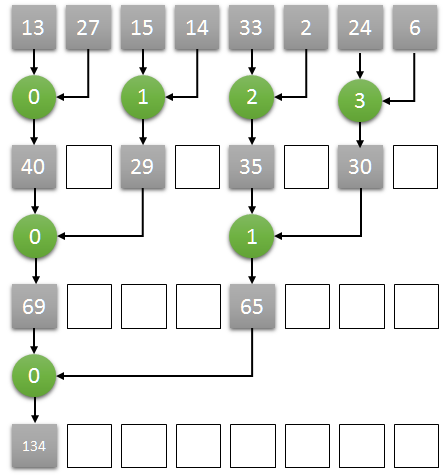
\includegraphics[scale=0.5]{imagenes/parallel_reduce.png}
\caption{Una reducción paralela de una sumatoria en CUDA.}
\label{image:cudareduction}
\end{figure}


En la figura \ref{image:cudareduction} podemos observar un ejemplo en el que se ve la estrucutra de cómo sería una reducción paralela en CUDA para un pequeño ejemplo. Para más información sobre cómo realizar una implementación de alto rendimiento de esta operación en CUDA puede consultarse en \cite{reduction}.\\

En nuestro trabajo la operación a la que queremos aplicar la reducción es el mínimo sobre un largo array de distancias. La operación mínimo \textbf{cumple la propiedad asociativa}, es decir:

$$min(min(a,b), c) = min(a, min(b, c))
$$

Además, si en vez pasar el valor para realizar la operación utilizamos un puntero en la memoria del dispositivo. Tras realizar toda la reducción con utilizar aritmética de punteros y restar al puntero inicial el puntero del valor mínimo obtenemos la solución deseada de forma eficiente. Una vez comprendido lo que esta operación implica, hemos decidido utilizar la función argmin de la librería CuPy que actúa de la forma comentada pero se encuentra altamente optimizada ofreciéndonos un gran rendimiento.

\begin{code}
\begin{minted}[fontsize=\footnotesize]{python}
import cupy as cp
min_index = cp.argmin(distances)
\end{minted}
\captionof{listing}{CuPy: Reducción para encontrar índice mínimo.\\}
\label{code:cupyreduce}
\end{code}


\subsubsection{Actualizar la BMU y su vecindario.}
Para esta operación necesitamos una vez tenemos encontrada la BMU actualizar una región alrededor de la misma y dependiente del parámetro de control $\sigma$, que controlaba el tamaño del vecindario. Recordemos que el parámetro $\sigma$ empezaba con un valor muy alto que se iba reduciendo exponencialmente y luego era fijado a otro parámetro indicado por el usuario, que debería de ser muy pequeño. Esto hace que en las primeras iteraciones se actualicen muchas neuronas y conforme vamos avanzando bastante menos. Los beneficios a la hora de paralelizar la actualización del mapa de neuronas de ese valor de $\sigma$, pues a mayor valor mayor es el número de neuronas alrededor que debemos evaluar. En esta implementación, hemos considerado siempre utilizar \textit{CUDA} para realizar la actualización pero sería una alternativa perfectamente viable utilizar la CPU en los casos en los que $\sigma$ es bajo y sólo un número pequeño de neuronas es afectado y el traslado de los datos necesarios de la matriz de pesos, que se encuentra en la GPU, de dispositivo a host y luego de vuelta no suponga un \textit{overhead} demasiado caro.\\

En la implementación que nosotros hemos realizado, que se corresponde a otro kernel de \textit{Numba} (código fuente \ref{code:updateonline}), cada hebra lanzada se corresponde a una neurona. Cada neurona comprueba su distancia con respecto a la BMU y si dicha distancia es válida procede a actualizar los datos que le corresponden conforme a la ecuación de actualización de pesos.

\begin{code}
\begin{minted}[fontsize=\footnotesize]{python}
@cuda.jit
def bmu_update(ids, samples, weights, d, bmu_row, 
    bmu_col, cols, eta, sigma_squared):
  idx = cuda.grid(1)
      if idx * d < weights.size:
          
          # 1. Medimos la distancia en la matriz del elemento actual a la BMU
          
          current_row = idx // cols
          current_col = idx % cols

          d_f = (current_col - bmu_col) * (current_col - bmu_col)
          d_f += (current_row - bmu_row) * (current_row - bmu_row)
          if d_f <= sigma_squared:
              # 2. Actualizamos acorde a esa distancia y el valor de sigma
              d_f = math.exp(-d_f/(2*sigma_squared))
              for i in range(d):
                  weights[idx * d + i] += eta * d_f * \
                  (samples[ids * d + i] - weights[idx * d + i])
\end{minted}
\captionof{listing}{Numba: Actualización de pesos de neuronas}
\label{code:updateonline}
\end{code}

\subsubsection{Actualizar los parámetros de control.}
Los parámetros de control $\eta$ y $\sigma$ son sólo dos parámetros a modificar por iteración y cuyo cálculo no es excesivamente complejo, razón por la que no es lo ideal paralelizar esta subproblema en la GPU y esto será realizando en la CPU, que, además puede realizar dicha operación de manera asíncrona mientras se está ejecutando alguno de los \textit{kernels}.

\subsubsection{Diagrama de flujo de la solución implementada.}
\begin{figure}[ht]
\centering
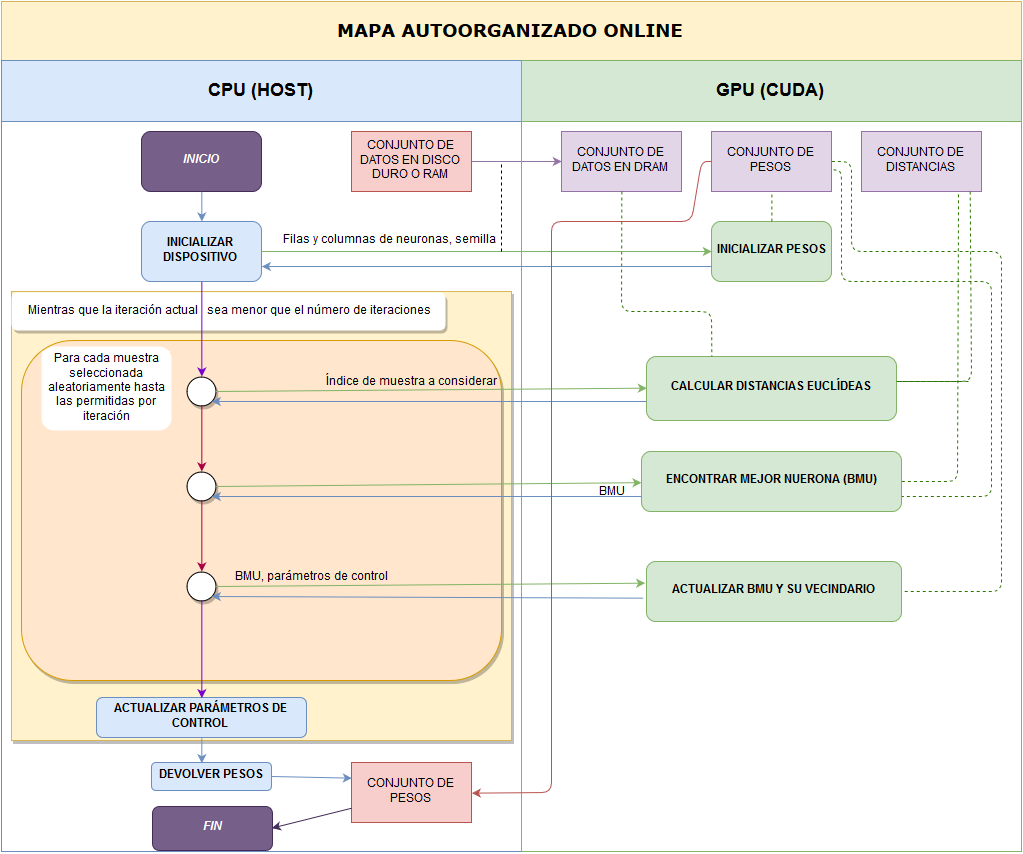
\includegraphics[scale=0.35]{imagenes/flujosomonline.png}
\caption{Diagrama de flujo para el mapa autoorganizado online.}
\end{figure}


\subsection{Desarrollo del mapa autoorganizado batch.}
En la versión \textit{batch} del algoritmo, aparece la posibilidad de evaluar múltiples muestras a la vez con el cambio de la ecuación de actualización de pesos. Ahora, en cada iteración los pesos de una neurona son la media de las muestras que lo activan y las que activan a las neuronas cercadas ponderada según la distancia en el vecindario del mapa. De manera similar a la sección anterior podemos subdividir el problema en pequeños subproblemas a resolver pero paralelizando en función del número de muestra en vez del de neuronas.

\begin{itemize}
  \item 1. Inicialización aleatoria de la matriz de pesos.
  \item 2. Cálculo de las distancias euclídeas entre todas las muestras y los pesos.
  \item 3. Encontrar la BMU para cada muestra.
  \item 4. Actualizar la matriz de pesos.
  \item 5. Actualizar los parámetros de control.
\end{itemize}

Tanto la \textbf{inicialización de la matriz de pesos} como la \textbf{actualización de los parámetros de control} son exáctamente \textbf{idénticas a la versión anterior} con ligeras variaciones, como que, por ejemplo, en la versión \textit{batch} no utilizamos la tasa de aprendizaje $\eta$ porque no es necesaria para obtener buenos resultados.\\

Para el \textbf{cálculo de las distancias euclídeas} necesitamos cambiar la idea planteada anteriormente puesto que ahora tenemos que evaluar todas las muestras con todas las neuronas. 
En este caso se lanzan tantas hebras como sea el producto del número de neuronas y el número de muestras, calculando cada hebra la distancia euclídea entre la muestra y la neurona que les corresponden. De manera similar a la anterior versión, obviamos el cálculo de la ráiz cuadrada. Puesto que ahora tenemos que evaluar todas las muestras a la vez no hemos planteado uso alguno de la memoria compartida para permitir que la solución sea aplicable a problemas de diversas características, pero si sabemos que la dimensión de una muestra del conjunto de datos no es excesivamente grande podríamos utilizar la memoria compartida para trabajar con los pesos del mapa. El código fuente \ref{code:euclideanbatch} muestra la implementación de este kernel en Numba.

\begin{code}
\begin{minted}[fontsize=\footnotesize]{python}
@cuda.jit
def batch_euclidean_distance(samples, weights, distances):
  idx = cuda.grid(1)
    if idx < distances.size:
        nrows, ncols, d = weights.shape
        nneurons = nrows * ncols
        row = idx // nneurons
        col = idx % nneurons
        wrow = col // ncols
        wcol = col % ncols

        my_distance = 0
        for i in range(d):
            i_distance = samples[row,i] - weights[wrow, wcol, i]
            my_distance += i_distance * i_distance
            
        distances[row, col] = my_distance
\end{minted}
\captionof{listing}{Numba: Distancia euclídea entre todas las muestras y neuronas.\\}
\label{code:euclideanbatch}
\end{code}

El proceso para \textbf{encontrar las BMU} vuelve a ser bastante similar utilizando la reducción. Sin embargo, ahora debemos de lanzar $N$ reducciones consecutivas para obtener la BMU de cada muestra. Utilizando CuPy podemos indicar si queremos hacer la reducción a lo largo de uno de los ejes, como se ve en el código fuente \ref{code:cupyreduce2}.

\begin{code}
\begin{minted}[fontsize=\footnotesize]{python}
import cupy as cp
# Se reduce cada fila
min_index = cp.argmin(distances, axis=1)
\end{minted}
\captionof{listing}{CuPy: Reducción para encontrar índice mínimo a lo largo de un eje en una matriz bidimensional.\\}
\label{code:cupyreduce2}
\end{code}

La parte más compleja de resolver en la versión \textit{batch} del algoritmo es la \textbf{actualización de la matriz de pesos}. Recordemos que en cada iteración, para obtener el nuevo vector de pesos hemos de aplicar la ecuación.

$$
 W_{i, j} = \frac{\sum_{k=0}^{f} \delta_f(c, [i,j]) \cdot X(T_k) }{\sum_{k=0}^{f} \delta_f(c, [i,j])}
$$\\

Por tanto, las neuronas que han sido activadas han de ser actualizadas en funcion de sus pesos. La solución que hemos planteado se basa en que primero se calculen las sumatorias del numerador y el denominador y posteriormente se pase otro kernel para hacer la división. Dado que al paralelizarlo existe la posibilidad de que múltiples hebras nos encontraríamos ante una condición de carrera lo que nos deja tres alternativas para resolver este problema.

\underline{Alternativas disponibles.}
\begin{itemize}
  \item a) Utilizar las operaciones de suma atómica del dispositivo.
  \item b) Utilizar una estructura auxiliar más grande y realizar reducciones sobre ella.
  \item c) Resolver este problema en la CPU.
\end{itemize}

La {opción a} fua la primera en ser implementada. El proceso se divide en dos \textit{kernels} uno que se encarga de generar los numeradores y denominadores para la fórmula de actualización nueva de cada neurona y otro que se encarga de hacer la división entre numerador y denominador para actualizar los pesos.\\

En el primero de estos \textit{kernels} (código fuente \ref{code:numbanumdem}) utilizamos la operación de suma atómica, esta operación es capaz de leer y escribir sobre una posición de memoria de la GPU en una única operación sin interferencia de ninguna otra hebra, lo que nos permite evitar el problema inicial limitando el rendimiento pero necesario para obtener resultados correctos. En la implementación propuesta, cada hebra se encargará de tomar la BMU de una muestra y actualizar su vecindario. 

\begin{code}
\begin{minted}[fontsize=\footnotesize]{python}
@cuda.jit
def prepare_update(bmu_row, bmu_col, samples, num, den, 
    nrows, ncols, sigma_squared):
  idx = cuda.grid(1)
    if idx < bmu_row.size:
        my_row = bmu_row[idx]
        my_col = bmu_col[idx]
        
        init_row = max(0, my_row - int(sigma_squared))
        finish_row = min(nrows, my_row + int(sigma_squared) + 1)
        
        init_col = max(0, my_col - int(sigma_squared))
        finish_col = min(ncols, my_col + int(sigma_squared) + 1)
        
    
        for i in range(init_row, finish_row):
            for j in range(init_col, finish_col):
                dist = (j-my_col) * (j-my_col) + (i-my_row) * (i-my_row)
    
                if dist <= sigma_squared:
                    hck = math.exp(-(dist)/(2 * sigma_squared))
                    cuda.atomic.add(den, i*ncols+j, hck)
                    d = samples.shape[1]
                    for k in range(d):
                        cuda.atomic.add(num, i*ncols*d + j*d +k,
                        hck * samples[idx, k])
\end{minted}
\captionof{listing}{Numba: Cálculo de numerador y denominador de la ecuación mediante suma atómica.\\}
\label{code:numbanumdem}
\end{code}

En el segundo kernel (código fuente \ref{code:numbaweightsbatch}), lanzamos tantas hebras como neuronas haya y actualizamos los pesos de cada neurona en función de los numeradores y denominadores calculados en el kernel anterior. Si esa neurona no se ha visto afectada en el cálculo de numeradores y denominadores, se mantiene los pesos de la iteración anterior.
\begin{code}
\begin{minted}[fontsize=\footnotesize]{python}
@cuda.jit
def finish_update(weights, num, den):
  idx = cuda.grid(1)
    if idx < den.size:
        nrows, ncols, d = weights.shape
        row = idx // ncols
        col = idx % ncols
        my_den = den[row * ncols + col]
        if my_den != 0:
            for k in range(d):
                weights[row, col, k] = num[row*ncols*d + col*d +k] / my_den
      
        cuda.syncthreads()
       
        for k in range(d):
            num[row*ncols*d + col*d +k] = 0
            
        den[row * ncols + col] = 0
\end{minted}
\captionof{listing}{Numba: Actualización de pesos en función de numeradores y denominadores.\\}
\label{code:numbaweightsbatch}
\end{code}


El procedimiento será mucho más costoso en las primeras iteraciones y menos costoso conforme se avance al irse reduciendo el vecindario. Para evaluar el rendimiento de esta versión utilizamos el profiler de NVIDIA, \textbf{nvprof} para medir el tiempo que se tarda en obtener los resultados de esta forma así como el tiempo que ha tardado en ejecutarse el algoritmo. Para realizar el profile hemos utilizado el conjunto de datos de las caras de \textit{Olivetti} (explicado en el siguiente capítulo). En la tabla \ref{tab:batchprofileparams} podemos observar los parámetros de control utilizados para la ejecución de este ejemplo.

\begin{table}[ht]
\begin{tabular}{|l|l|l|l|l|l|l|l|}
\hline
\multicolumn{1}{|c|}{\textbf{Muestras}} & \textbf{Dimensión} & \multicolumn{1}{c|}{\textbf{Neuronas}} & \textbf{Épocas} & \textbf{\begin{tabular}[c]{@{}l@{}}Épocas\\ 1º Fase\end{tabular}} & $\sigma_0$ & $\sigma_f$ & $\tau$ \\ \hline
400                                     & 4096               & 400 (20x20)                            & 400             & 100                                                               & 15         & 0.1        & 400    \\ \hline
\end{tabular}
\caption{Parámetros de control para el ejemplo utilizando en el profiler.}
\label{tab:batchprofileparams}
\end{table}


Los resultados más relevantes proporcionados por el profiler se encuentran en la tabla \ref{tab:batchprofile}.\\

\begin{table}[ht]
\centering
\begin{tabular}{|l|l|crrr}
\hline
\rowcolor[HTML]{EFEFEF} 
\multicolumn{1}{|c|}{\cellcolor[HTML]{EFEFEF}\textbf{Actividad}}                                                  & \multicolumn{1}{c|}{\cellcolor[HTML]{EFEFEF}\textbf{\begin{tabular}[c]{@{}c@{}}Tiempo\\ total\end{tabular}}} & \multicolumn{1}{c|}{\cellcolor[HTML]{EFEFEF}\textbf{\begin{tabular}[c]{@{}c@{}}Nº\\usos\end{tabular}}} & \multicolumn{1}{c|}{\cellcolor[HTML]{EFEFEF}\textbf{\begin{tabular}[c]{@{}c@{}}Mín\end{tabular}}} & \multicolumn{1}{c|}{\cellcolor[HTML]{EFEFEF}\textbf{\begin{tabular}[c]{@{}c@{}}Medio\end{tabular}}} & \multicolumn{1}{c|}{\cellcolor[HTML]{EFEFEF}\textbf{\begin{tabular}[c]{@{}c@{}}Máx\end{tabular}}} \\ \hline
\rowcolor[HTML]{EFEFEF} 
\cellcolor[HTML]{F8A102}\textbf{CPU + GPU}                                                                        & \cellcolor[HTML]{F8A102}56,62 s                                                                              & \multicolumn{1}{l}{\cellcolor[HTML]{EFEFEF}}                                                               & \multicolumn{1}{l}{\cellcolor[HTML]{EFEFEF}}                                                                  & \multicolumn{1}{l}{\cellcolor[HTML]{EFEFEF}}                                                                  & \multicolumn{1}{l}{\cellcolor[HTML]{EFEFEF}}                                                                  \\ \cline{1-2}
\rowcolor[HTML]{EFEFEF} 
\cellcolor[HTML]{38FFF8}\textbf{GPU}                                                                              & \cellcolor[HTML]{38FFF8}55,37 {[}100 \%{]}                                                                   & \multicolumn{1}{l}{\cellcolor[HTML]{EFEFEF}}                                                               & \multicolumn{1}{l}{\cellcolor[HTML]{EFEFEF}}                                                                  & \multicolumn{1}{l}{\cellcolor[HTML]{EFEFEF}}                                                                  & \multicolumn{1}{l}{\cellcolor[HTML]{EFEFEF}}                                                                  \\ \hline
\rowcolor[HTML]{ECF4FF} 
\textbf{\begin{tabular}[c]{@{}l@{}}Cálculo de\\ distancias\end{tabular}}                                          & 14,67 s {[}26,5 \%{]}                                                                                        & \multicolumn{1}{c|}{\cellcolor[HTML]{ECF4FF}400}                                                           & \multicolumn{1}{r|}{\cellcolor[HTML]{ECF4FF}35,67 ms}                                                         & \multicolumn{1}{r|}{\cellcolor[HTML]{ECF4FF}35,68 ms}                                                         & \multicolumn{1}{r|}{\cellcolor[HTML]{ECF4FF}45,58 ms}                                                         \\ \hline
\rowcolor[HTML]{ECF4FF} 
\textbf{\begin{tabular}[c]{@{}l@{}}Encontrar \\ BMUs\end{tabular}}                                                & 23,78 ms {[}0,04 \%{]}                                                                                       & \multicolumn{1}{c|}{\cellcolor[HTML]{ECF4FF}400}                                                           & \multicolumn{1}{r|}{\cellcolor[HTML]{ECF4FF}54,82 $\mu$s}                                                     & \multicolumn{1}{r|}{\cellcolor[HTML]{ECF4FF}59,47 $\mu$s}                                                     & \multicolumn{1}{r|}{\cellcolor[HTML]{ECF4FF}68,26 $\mu$s}                                                     \\ \hline
\rowcolor[HTML]{ECF4FF} 
{\color[HTML]{CB0000} \textbf{\begin{tabular}[c]{@{}l@{}}Generar \\ numeradores y \\ denominadores\end{tabular}}} & {\color[HTML]{FE0000} \textbf{39,97 s {[}72,19 \%{]}}}                                                       & \multicolumn{1}{c|}{\cellcolor[HTML]{ECF4FF}400}                                                           & \multicolumn{1}{r|}{\cellcolor[HTML]{ECF4FF}1,05 ms}                                                          & \multicolumn{1}{r|}{\cellcolor[HTML]{ECF4FF}99,93 ms}                                                         & \multicolumn{1}{r|}{\cellcolor[HTML]{ECF4FF}458,2 ms}                                                         \\ \hline
\rowcolor[HTML]{ECF4FF} 
\textbf{\begin{tabular}[c]{@{}l@{}}Actualizar \\matriz  de pesos\end{tabular}}                                    & 695,01 ms {[}1,26 \%{]}                                                                                      & \multicolumn{1}{c|}{\cellcolor[HTML]{ECF4FF}400}                                                           & \multicolumn{1}{r|}{\cellcolor[HTML]{ECF4FF}1,68 ms}                                                          & \multicolumn{1}{r|}{\cellcolor[HTML]{ECF4FF}1,74 ms}                                                          & \multicolumn{1}{r|}{\cellcolor[HTML]{ECF4FF}1,86 ms}                                                          \\ \hline
\end{tabular}
\caption{Resumen de tiempos más importantes de la ejecución del profiler.}
\label{tab:batchprofile}
\end{table}

Podemos observar que el cuello de botella en esta ejecución es el kernel asociado a computar los numeradores y denominadores, ocupando el 72 \% del tiempo de ejecución de la CPU. Por ello, vamos a analizar el resto de opciones para ver cuál es su rendimiento.

La \textbf{opción b} fue descartada pues conllevaría serían necesarias dos estructuras auxiliares para almacenar los numeradores y los denominadores. En el caso en cuestión, necesitaríamos 2,5 GiB para los numeradores y 625 KiB que generan una complejidad espacial excesiva.\\

Dados los resultados de la opción a, hemos decidido probar también a implementar la \textbf{opción c}. En esta versión, el cálculos de distancias y encontrar la BMU es realizado en la GPU y la actualización de pesos en la CPU con el fin de evaluar si el gran porcentaje de tiempo que se tarda es por la dificultad del problema o porque las operaciones atómicas del dispostivo \textit{CUDA} no son lo suficientemente eficientes. Tras evaluarlo empíricamente, el tiempo total de ejecución de esta opción alcanzó los 160,56 segundos que es mucho más lento que los 56,62 segundos de la opción a. Por tanto, esta opción también fue descartada y nos quedamos con la implementación inicial utilizando la suma atómica.


\subsubsection{Diagrama de flujo de la solución final implementada.}

\begin{figure}[ht]
\centering
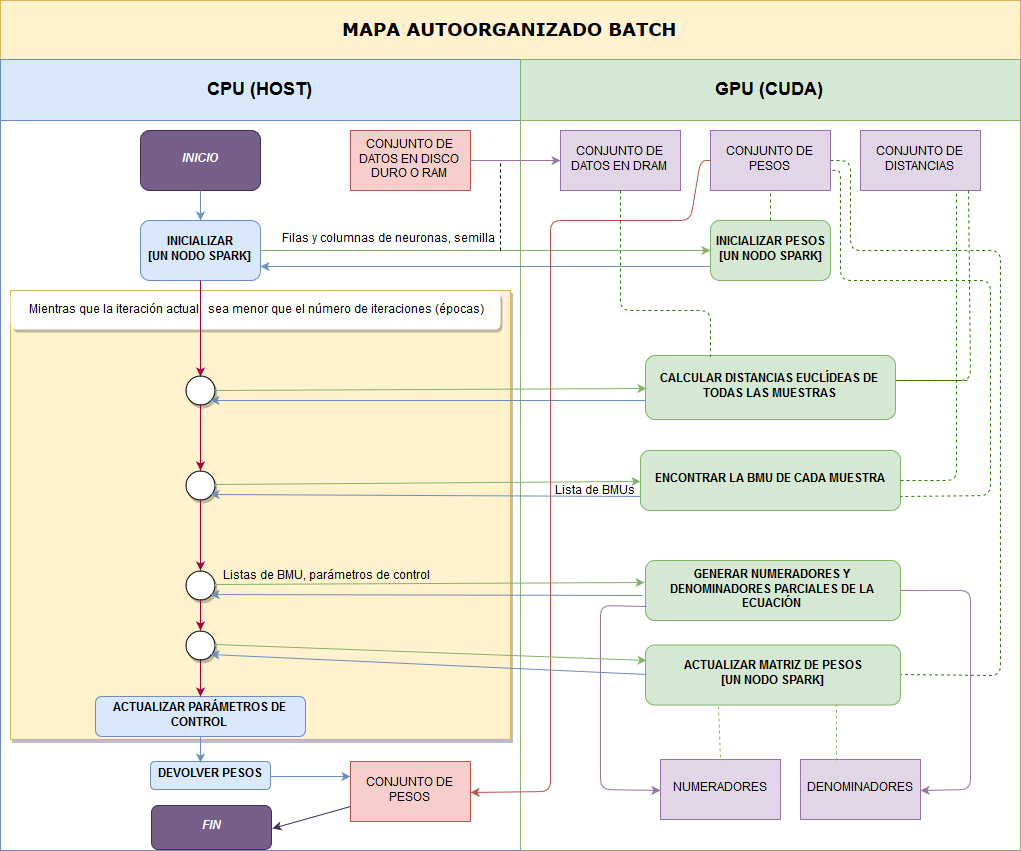
\includegraphics[scale=0.35]{imagenes/flujosombatch.png}
\caption{Diagrama de flujo para el mapa autoorganizado batch.}
\end{figure}
\chapter{Modelos de Soft Computing considerados.}
\section{Mapas autoorganizados \textit{(Self Organizing Map)}}
A principio de la década de los 80 el científico finlandés Teuvo Kohonen \cite{kohonensom} planteó un modelo de aprendizaje automático no supervisado y competitivo basándose en el funcionamiento del estudio del córtex cerebral. El modelo planteado, denominado mapa autoorganizado, red autoorganizada o red neuronal de Kohonen, entre otros nombres similares, es una red neuronal artificial, y las principales características que la define son las siguientes:

\begin{itemize}
	\item Es una \textbf{red neuronal artificial}. Esto quiero decir, a grandes rangos, que la estructura que genera el modelo está basada en una red de múltiples neuronas que se encuentra interconectadas entre sí.
	
	\item La red neuronal de Kohonen tiene \textbf{dos capas}. Una capa de entrada, con tantas neuronas como características tenga una muestra a ser evaluada por la red, y una capa de salida de un tamaño que decide el usuario. Habitualmente, esta capa de salida, también llamada capa competitiva o capa de Kohonen, presenta una distribución bidimensional, aunque podría perfectamente usarse cualquier otro número de dimensiones.

	\item Cada neurona de la capa de entrada está asociada con todas las neuronas de la capa de salida y las neuronas de la capa de salida no están interconectadas entre sí. A este tipo de red neuronal, en la que no existen ciclos, se le denomina \textbf{red neuronal prealimentada} \textit{(feed-forward)}.

	\item Asociada a cada neurona de la capa de salida, tenemos un vector de pesos sinápticos obtenido a través de las conexiones con la capa de entrada que es modificado durante el proceso de aprendizaje. A dicho vector de pesos se le llama vector de referencia y representa el valor promedio de la categoría asociada a esa neurona. El conjunto de todos esos vectores de referencia es denominado \textit{codebook}.

	\item Es un algoritmo \textbf{no supervisado} capaz de encontrar patrones comunes basándose en los datos de la muestra de entrada sin necesidad de que cuando una muestra entre a la red se indique a qué categoría pertenece.

	\item Es un modelo \textbf{competitivo}. Cuando se recibe una muestra todas las neuronas compiten por ser activadas pero sólo la mejor será activada.
\end{itemize}

\begin{figure}
\centering
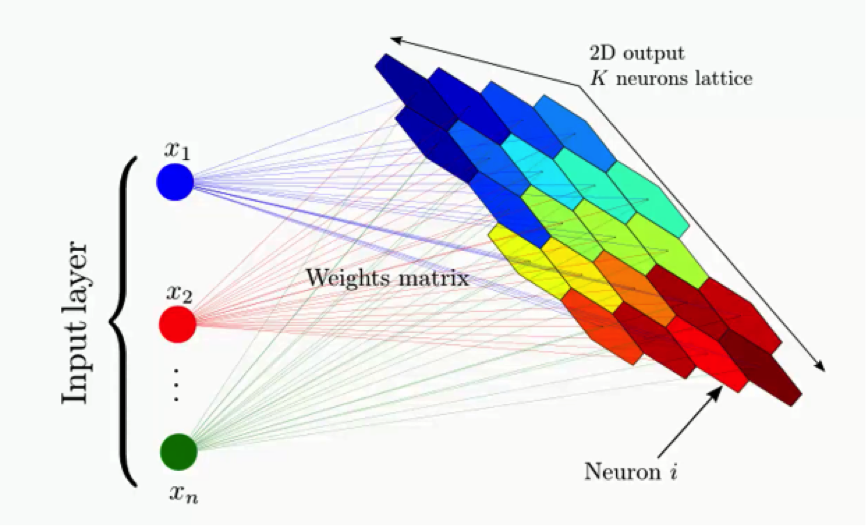
\includegraphics[width=0.8\textwidth]{imagenes/arquitectura_som.png}
\caption{Esquema de una red neuronal de Kohonen.}
\end{figure}

\subsection{Proceso de entrenamiento.}

En primer lugar, se \textbf{inicializan} \textbf{los pesos} asociados a la capa de salida. Lo más habitual, es tomar dichos pesos de una distribución aleatoria.
Para un correcto funcionamiento dichos pesos deben estar normalizados entre 0 y 1. En nuestro caso, hemos tomado los pesos de una distribución aleatoria uniforme en el intervalo $[0, 1)$.\\

El proceso de entrenamiento que se presenta a continuación \textbf{se repite hasta que se alcanza el número de iteraciones máximo}, determinado por el parámetro $\lambda$. La variable $t$ representa cada una de las iteraciones.\\

Después, para cada una de las muestras, $X$, sacadas de la distribución de muestras, de forma aleatoria, se realizan los siguientes pasos: \\\\
1 - Se \textbf{calcula la distancia euclídea} entre la muestra $X$ y cada una de las neuronas de la capa de salida. También se pueden utilizar otro tipo de distancias.\\
$$distancia(X) = || W - X ||$$\\
2 - Se \textbf{busca la neurona que ha obtenido una menor distancia}. Esta neurona es considerada la neurona ganadora o BMU \textit{(Best Matching Unit)}.\\
$$BMU_X = argmin_{W_{i, j}} \; distancia(X) = argmin_{W_{i, j}} || W - X ||$$\\

La función \textit{argmin} devuelve el índice del array en el que se alcanza el valor mínimo.

3 - Se realiza un \textbf{proceso de actualización de las matrices de pesos} en base a lo obtenido anteriormente, según la siguiente fórmula.\\
$$ W_{i, j}^{(t+1)} = W_{i, j}^{(t)} + \Delta {W_{i,j}} $$\\

La actualización depende tanto de la distancia de la muestra al vector de pesos como de otros dos parámetros: la tase de aprendizaje y una función de vecindario.\\

$$\Delta W_{i,j} = \eta(t)\delta_f(i,j)(X-W_{i,j})$$\\

La función $\delta_f(i,j)$ es la función de vecindario y, en nuestra propuesta, se calcula conforme a la siguiente función gaussiana:\\

$$\delta_f(i,j) = e ^{-\frac{||BMU_X-(i,j)||^2}{2\sigma(t)^2}}. $$\\

Al tratar con una potencia con exponente negativo, un mayor valor absoluto de dicho exponente nos proporciona una valor de $\delta_f(i,j)$ menor. Por eso en el numerador se tiene en cuenta la distancia que hay entre la mejor neurona y la neurona actual. En el denominador se utiliza un parámetro de control $\sigma$que nos permite controlar la distancia que estamos considerando.\\\\

Normalmente, este parámetro, durante un primer número de iteraciones previamente proporcionado, es inicializado a un valor alto $\sigma_0$ que decrece de manera exponencial conforme a otro parámetro de control $\tau$.

Una vez ha finalizado esa primera fase (han pasado $z$ iteraciones) se van refinando los resultados con un valor fijo mucho más bajo $\sigma_f$.\\


$$\sigma(t) = \left\{
\begin{array}{ll}
\sigma_0e^{-\frac{t}{\tau}} & si \;\;t < z\\
\sigma_f & si  \;\; t\geq z
\end{array}
\right.
$$\\

Para la tasa de aprendizaje se sigue una aproximación similar, la tasa de aprendizaje durante la primera fase está inicializada a un valor $\eta_0$ decreciendo conforme a una función gaussiana y, una vez pasado un número de iteraciones, se fija a un valor $\eta_f$. \\
$$\sigma(t) = \left\{
\begin{array}{ll}
\eta_0e^{-\frac{t}{\tau}} & si \;\;t < z\\
\eta_f & si  \;\; t\geq z
\end{array}
\right.$$\\

Así pues, este algoritmo acerca los pesos del vecindario de la BMU hacia la nueva muestra introducida para parecerse más a la misma. Esto lo hace teniendo en cuenta un vecindario alrededor de la BMU que decrece exponencialmente conforme pasa un número de iteraciones hasta quedarse fijo y una tasa de aprendizaje que también decrece exponencialmente hasta permanecer constante. \\

Esto permite una primera fase de entrenamiento, con cambios más bruscos en la que se adaptan los valores completamente aleatorios para encontrar agrupamientos razonables. Conforme avanza dicha fase esos valores van decreciendo, hasta que quedan fijados permitiendo a la red neuronal refinar los agrupamientos obtenidos hasta ese momento.\\

\subsection{Usos del mapa autoorganizado.}
El modelo del mapa autoorganizado puede ser utilizado para diversas tareas, de entre las que destacan:

\begin{itemize}
	\item \textbf{Clustering} - es decir, generar agrupaciones del conjunto de datos de entrada. Por regla general, cada neurona de la capa de Kohonen representaría una posible agrupación de los datos. 

	\item \textbf{Visualización de datos de alta dimensionalidad.} Tras finalizar el proceso de entrenamiento, podemos utilizar diferentes técnicas para obtener una representación visual de las características topológicas de la muestras. Las matrices-U, las matrices-P o los planos de componentes son algunos de los modelos utilizados para visualizar el mapa autoorganizado.

	\item \textbf{Clasificación.} Una vez terminado el proceso de entrenamiento, puede asignarse etiquetas a cada uno de los nodos y resolver problemas de clasificación dependiendo de qué BMU se active. 
	\end{itemize}

\subsection{Mapa autoorganizado batch.}
El proceso de entrenamiento previamente mencionado se corresponde al del mapa autoorganizado tradicional u \textit{online}. En ese proceso, durante una iteración, se evalúa un subconjunto de los datos como parte de un proceso secuencial de encontrar la BMU y actualizar los pesos correspondientes. Posteriormente, basándose en las propiedades matemáticas del mapa autoorganizado \textit{online}, se derivó una formulación para realizar el proceso de actualización de pesos en una sola iteración para un bloque de muestras. Esta versión del algoritmo, es denominada mapa autoorganizado \textit{batch}. \\

En esta versión, la regla para la actualización de pesos implica que durante cada iteración, los pesos de las neuronas sean actualizados con la media de las muestras que lo activan teniendo en cuenta los parámetros de control como el vecidario o la tasa de aprendizaje. $T_0$ representa el inicio de una época y $T_f$ el final de la misma. En cada instante $T_k$ de una época se evalúa una muestra $X(T_k) $del conjunto de datos. La nueva fórmula para la actualización de los pesos es la siguiente:\\

$$
 W_{i, j} = \frac{\sum_{k=0}^{f} \delta_f(c, [i,j]) \cdot  X(T_k) }{\sum_{k=0}^{f} \delta_f(c, [i,j])}
$$\\

donde $c$ es la unidad de activación (BMU) para la muestra $X(T_i)$ y permitiéndose obviar el parámetro $\eta(t)$ que controlaba la tasa de aprendizaje.\\

El uso del modelo \textit{batch} frente al modelo tradicional conlleva un intercambio de ventajas e incovenientes \cite {compsom} que podemos observar en la tabla \ref{tab:somcomparative}.

\begin{table}[ht]
\begin{tabular}{|l|l|}
\hline
\multicolumn{1}{|c|}{\textit{\textbf{Ventajas}}}                                                                                  & \multicolumn{1}{c|}{\textit{\textbf{Inconvenientes}}}                                                    \\ \hline
Mayores oportunidades de paralelización.                                                                           & \multirow{2}{*}{\begin{tabular}[c]{@{}l@{}}Peor organización topográfica\\ y visualización\end{tabular}} \\ \cline{1-1}
Converge más rápido que el tradicional.                                                                                               &                                                                                                          \\ \hline
El parámetro $\eta$ es opcional.                                                                                                  & Puede salir clases muy desbalanceadas.                                                                   \\ \hline
\begin{tabular}[c]{@{}l@{}}Resultados deterministas, excepto la\\ inicialización si se ha realizado\\ aleatoriamente.\end{tabular} & Alta dependencia de la inicialización                                                                    \\ \hline
\end{tabular}
\caption{Ventajas e incovenientes de la versión batch}
\label{tab:somcomparative}
\end{table}





\subsection{Medidas de calidad.}
Para medir la calidad de un mapa autoorganizado una vez entrenado podemos utilizar dos medidas:\\

El \textbf{error medio de cuantificación} nos permite medir la precisión del mapa creado. Se calcula tomando la media de las distancias euclídeas entre cada una de las muestras y su correspondiente BMU.\\

$$
\epsilon_q = \frac{1}{N}\sum_{i=1}^{N}  || x_i - codebook[BMU(x)] ||
$$\\

El \textbf{error topográfico} mide la capacidad que ha tenido el modelo de conservar las propiedades topográficas del conjunto de muestras de entrenamiento. Podemos medir dicho error como:\\
$$
u(x_k) = \left\{
\begin{array}{ll}
1 & si \; su \; BMU \; y \; la \; segunda \; BMU \; son \; adyacentes.\\
0 & en \; caso \; contrario.
\end{array}
\right.
$$
$$
\epsilon_t =  \frac{1}{N}\sum_{i=1}^{N} u(x_k)
$$\\

\newpage
\section{Árboles de decisión.}
Un árbol de decisión \cite{arbol} es un modelo de aprendizaje automático supervisado utilizado para resolver problemas de clasificación y extensible para resolver problemas de regresión. Un árbol de decisión, una vez entrenado, consiste en una estructura jeráquica de reglas que nos indica a qué categoría pertenece una muestra del conjunto de datos de entrada. Dicho árbol está formado por dos tipos de nodos:
\begin{itemize}
	\item Los \textbf{nodos de decisión}. En dichos nodos existe una pregunta sobre un atributo y valor (o varios) y dependiendo de la respuesta se toma el camino asociado a ésta que parte de este nodo de decisión y nos lleva a otro nodo del árbol.
	\item Los \textbf{nodos terminales} o nodos respuesta nos indican la clase, o el valor en caso de árboles de regresión, a la que ha de pertenecer si al evaluar una muestra dicho nodo ha sido alcanzado. Estos nodos se corresponden con las hojas del árbol formado.
\end{itemize}


\subsection{Proceso de entrenamiento.} 

Obtener un árbol de decisión óptimo es un problema \textbf{NP-completo}, es decir, no se conoce manera de resolver este problema con una complejidad de tiempo polinómico por lo que es habitual que los algoritmos que realizan el entrenamiento de este modelo sigan estrategias voraces \textit{(greedy)}. Los algoritmos más conocidos y utilizados para realizar esta tarea(ID3, CART, C4.5, C5.0) siguen un esquema de entrenamiento similar. \\

La idea que sigue el proceso de entrenamiento es realizar una serie de particiones binarias sobre el conjunto de datos inicial calculando todos los posibles puntos de corte de la partición y evaluando el mejor punto de corte existente. Este proceso es repetido hasta terminar de evaluar el árbol o que alguna de las condiciones de finalización temprana se cumpla, si es que la hubiere.\\

Todas las posibles divisiones para una partición se basan en repartir todas las muestras basándose en un atributo y un valor asociado a un \textbf{punto de corte}. Si, para una muestra, su valor para el atributo en cuestión es inferior al valor del punto de corte, es asignada a una de las subdivisiones y, en caso contrario, es asignada a la otra subdivisión. Habitualmente, los puntos de corte son la media de entre un valor y su sucesor, considerando el conjunto de los valores del atributo ordenado y único, es decir, no se puede repetir un valor.\\

Cada una de estas posibles divisiones es evaluada conforme a diferentes criterios dependiendo del algoritmo, habitualmente basados en la impureza de cada una de las dos subdivisiones obtenidas al realizar el corte. 

La \textbf{ganancia de información} es una de las posibles medidas para determinar el mejor punto de corte de todos los posibles y se basa en la siguiente fórmula:

$$
GI(D,s) = Impureza(D) - \frac{|D_{izq}|}{|D|} \cdot Impureza(D_{izq}) - \frac{|D_{der}|}{|D|} \cdot Impureza(D_{der})
$$

donde $D$ es el conjunto de datos de la división actual, $s$ es el punto de corte y $D_{izq}$ y $D_{der}$ son las correspondientes subdivisiones obtenidas a partir del punto de corte.\\

Una medida de \textbf{impureza} \cite{impurity} es una función que, dada un conjunto de datos, mide la cantidad de clases distintas que hay en ese conjunto. Dicha medida valdrá 0 si todos los elementos pertenecen a la misma clase y 1 si cada elemento es de una clase distintas. En la tabla \ref{tab:entropy} destacamos algunas de estas medidas.\\

\begin{table}[ht]
\centering
\begin{tabular}{|l|l|l|}
\hline
\textbf{Impureza} & \textbf{Tarea} & \textbf{Fórmula}                         \\ \hline
\textbf{Entropía}  & Clasificación  & $\sum_{i=1}^{C}- f_i \cdot log (f_i)$    \\ \hline
\textbf{Gini}      & Clasificación  & $\sum_{i=1}^{C} f_i (1 - f_i)$           \\ \hline
\textbf{Varianza}  & Regresión      & $\frac{1}{N}\sum_{i=1}^|D|(y_i - \mu)^2$ \\ \hline
\end{tabular}
\caption{Algunas medidas de impureza.}
\label{tab:entropy}
\end{table}

donde $f_i$ es la probabilidad de pertenecer a la clase $i$ en una división, $C$ es el total de categorías únicas, $y_i$ es el valor del atributo a predecir de una instancia  y $\mu = \frac{1}{N} \sum_{i=1}^{N}y_i$ es la media de todas esos valores en una división.\\

\subsection{Poda de árboles y criterios de terminación temprana.}
Una de las principales cuestiones a la hora de generar un arbol de decisión es conocer cuál ha de ser el tamaño apropiado del mismo para que sea capaz de predecir de la mejor manera posible las muestras con las que se ha entrenado. Un árbol muy pequeño corre el riesgo de haber generalizado más de la cuenta la información procedente de las muestras, mientras que un árbol muy grande puede estar demasiado especializado, dejarse influir por ruido presente en las muestras y, como consecuencia, producir un sobreajuste de manera que cuando recibe nuevas muestras falla en las predicciones debido a ese gran nivel de especialización sobre el conjunto de entrenamiento. \\

Para evitar este tipo de problemas, es común recurrir a técncias de podado de árboles. Podemos distinguir dos tipos de técnicas de poda:

\begin{itemize}
	\item Técnicas de poda realizadas antes de que se termine de generar el árbol \textit{(pre-pruning)}.
	\item Técnicas de poda realizadas tras la construcción del árbol \textit{(post-pruning)}.
\end{itemize}

Las técnicas de poda \textit{pre-pruning} ayudan también a que la construcción del árbol finalice antes y, de entre ellas, destacamos:

\begin{itemize}
	\item Establecer un mínimo de elementos por nodo/partición, de manera que cuando se alcanza dicho umbral esa partición no sigue siendo evaluada.
	\item Establecer una profundidad máxima del árbol.
	\item Establecer algún criterio de ganancia de información mínima.
\end{itemize}

En el momento en que una de estas condiciones se cumple, dicho nodo se convierte en un nodo terminal. En el caso de los problemas de clasificación, es común realizar el voto mayoritario, donde se etiqueta una muestra con la clase más representativa del nodo, es decir la que tiene más instancias en el mismo. Por otro lado, en problemas de regresión es habitual etiquetar el nodo con la media de los valores a predecir ($\mu$) por el mismo.\\

De entre las técnicas de poda \textit{post-pruning} destacan dos:\\

La \textbf{poda de error reducido}. Esta poda utiliza una técnica simple y rápida de computar en la que, empezando por cada una de las hojas del árbol, se va sustituyendo cada nodo por la clase más popular. Si la predicción no ha empeorado, se continúa en los siguientes niveles de profundidad del árbol asociado al nodo en cuestión y, en el momento en la que dicha predicción empeora, el procedimiento termina.\\

La \textbf{poda de coste-complejidad}. En la poda de coste-complejidad se genera una serie de árboles $T_0, T_1, T_i, ... , T_r$ donde $T_0$ es el árbol inicial y $T_r$ es sólo la raíz. En cada iteración ($i$) del proceso, se elimina un subárbol del árbol anterior ($i-1$) reemplazándolo con un nodo terminal conforme al siguiente criterio:

$error(T, S)$ es el error del árbol $T$ sobre el conjunto de datos $S$. $poda(T, t)$ es el árbol obtenido de podar el subárbol $t$ del árbol $T$.\\

En cada iteración, se elimina el subárbol que minimiza:

$$
\frac{error(poda(T, t), S) - error(T, S)}{|hojas(T)| - |hojas(poda(T, t))|}
$$

Una vez generados todos los árboles $T_0$ a $T_r$ se selecciona aquel que proporciona una mayor precisión.\\

Generalmente, las técnicas de poda \textit{post-pruning} suelen dar mejores resultados pero son más costosas computacionalmente.
\subsection{Calidad del modelo.}
La principal medida de la calidad del modelo generado aparte de su tiempo de ejecución es la capacidad que tiene de predecir la clase correcta para una muestra. A dicha medida se le denomina \textbf{precisión}.

$$
Precision = \frac{1}{N}\sum_{i=1}{N}[1|f(x_i) = y_i]
$$

donde $f$ es la función que nos devuelve la clasificación proporcionada por el árbol de decisión, $x_i$ es cada una de las muestras a evaluar e $y_i$ es su correcta clasificación.

\subsection{Ventajas e incovenientes.}
\underline{Ventajas.}
\begin{itemize}
	\item Proporcionan un modelo de caja blanca fácil de interpretar y comprender.
	\item Puede ser combinado con otros modelos distintos o en un conjunto de árboles, por ejemplo, \textit{random forests}.
	\item No requieren de un gran preprocesamiento de las muestras antes de ser entrenados.
	\item A diferencia de otros modelos (como la regresión lineal), pueden resolver problemas de clasificación o regresión no lineales.\\
\end{itemize}

\underline{Incovenientes.}
\begin{itemize}
	\item Pequeños cambios en el conjunto de datos utilizado para el entrenamiento pueden alterar considerablemente los resultados obtenidos.
	\item Pueden proporcionar peores resultados que otros modelos no lineales (SVM, redes neuronales, etc) con los mismos datos pero, juntarlos en un ensemble, como los \textit{random forest} \cite{randomforest}, puede ayudarnos a solventar el problema, eso sí, eliminando la facilidad para interpretar el modelo que proporciona utilizar un único árbol.
	\item Encontrar el árbol de decisión óptimo global es un problema NP-completo.
\end{itemize}

%!TEX root = ../proyecto.tex
\chapter{Implementación.}
\section{Breve introducción a CUDA.}
Como comentábamos al principio, CUDA \textit{(Computer Unified Device Arquitecture)} \cite{cuda} es una tecnología propietaria desarrollada por \textit{NVIDIA} y lanzada en junio de 2007, que nos proporciona de un lenguaje de programación general destinado a ser ejecutado en las tarjetas gráficas de la compañia. Para los propósitos de este trabajo y, habitualmente, a la hora de trabajar con CUDA denominaremos como \textbf{\textit{host}} a la CPU que se comunica con la tarjeta gráfica y como \textbf{dispositivo} a la GPU o tarjeta gráfica utilizada. \\

La intercomunicación entre \textit{host} y dispositivo sigue un modelo maestro-esclavo. El \textit{host} actúa como maestro y es el encargado de indicar al dispoistivo el código que ha de ejecutar y de mandarlo a la cola del dispositivo. Además, el \textit{host} tiene la posibilidad de trabajar de forma asíncrona con la GPU mientras la cola de trabajos del dispositivo no esté llena. \\

Es de vital importancia a la hora de trabajar con la GPU de tener en cuenta que:\\
\begin{itemize}
    \item a) La GPU tiene muchos más núcleos \textit{(cores)} que una CPU, lo que nos permite realizar mucha más operaciones en el mismo instante. Sin embargo, esto viene a expensas de un menor número de operaciones por segundo de cada núcleo, ya que para distrutar de la cantidad masiva de núcleos que tiene una GPU es necesario que ésta opere a una frecuencia más baja.

    \item b) La GPU tiene su propia estructura de memoria, que ha de usar para poder realizar operaciones. Dentro de la jerarquía de memoria encontramos memoria RAM similar a la que utiliza la CPU a través de la placa base, así como varios niveles de caché. Además, hemos de tener en cuenta que a la hora de ejecutar algo en la GPU vamos a tener un gasto extra de tiempo por el traspaso de información de CPU a GPU y viceversa. Minimizar la información que ha de traspasarse en ambos sentidos así como intentar que toda la información necesaria sea transferida a la vez para sacar máximo potencial del PCI Express y exprimir al máximo posible el uso eficiente de la memoria caché, que en CUDA es habitualmente realizado mediante el manejo de la ``memoria compartida'' es fundamental para obtener mejores resultados, especialmente, aquellos en los que el cuello de botella es la transferencia de datos.

    \item c) Como la GPU tiene su propia memoria dedicada de un tamaño limitado hemos de hacer hincapié en no utilizar soluciones que generan demasiada complejidad espacial, ya que limitan la escalabilidad de los algoritmos.
\end{itemize}

\subsection{Estructura de hebras, bloques y mallas.}
El \textbf{\textit{kernel}} es un fragmento de código especial destino a ser ejecutado en el dispotivo en el que se indica lo que ha de hacer una hebra.\\

Las \textbf{hebras} son la unidad mínima en la arquitectura CUDA. Cada hebra es ejecutada por un núcleo CUDA. Cada hebra es consciente en tiempo de ejecución de su identificador dentro del bloque así como del identificador del bloque en el que se encuentra y el tamaño del mismo, permitiéndonos así repartir el trabajo en función de dichos valores. El \textbf{bloque} se corresponde a un conjunto de hebras que ejecuta el mismo \textit{kernel} y que pueden cooperar entre sí y, al conjunto de esos bloques, se le denomina \textbf{``grid'' o malla}. Tanto las hebras dentro de un bloque como los bloques dentro de una malla puede tener estructuras unidimensionales, bidimensionales y tridimensionales. Las dimensiones de estas estructuras será indicada por el \textit{host} a la hora de ejecutar el \textit{kernel}.\\

CUDA exige que un mínimo de 32 hebras, denominado \textit{warp}, ejecuten instrucciones a la vez, aunque se hagan cálculos innecesarios así como que todas las hebras de un bloque sean ejecutadas por el mismo \textit{Streaming MultiProcessor}, de ahora en adelante, SM, que es uno de los procesadores en el dispositivo y dispone de un número específico de núcleos CUDA, sus propios registros y su propia caché entre otros.\\

Al lanzar un \textit{kernel} hemos de utilizar al menos un bloque de $N$ hebras. Además, en los casos unidimensionales el número de hebras por bloque está limitado a un máximo que depende de la tarjeta gráfica en cuestión.

\subsection{La memoria compartida.}
Dentro de la tarjeta gráfica, nos encontramos con distintos niveles de memoria. Una vez los datos necesarios han sido traspasados del \textit{host} al dispositivo a través del bus PCI Express, esos datos son almacenados en una memoria DRAM de propósito general del dispositivo. Cuando un \textit{kernel} solicita datos de esta memoria, de manera similar a como ocurre en una CPU, los datos solicitados y los colidantes en memoria son colocados a través de varios niveles de caché, que tiene tamaño más limitado que la memoria DRAM pero con un acceso de lectura y escritura mucho más rápido.\\

La \textbf{memoria compartida} es una abstracción para una región especial de la caché asociada a un bloque que es explícitamente usada por el programador en el \textit{kernel}, agilizando así considerablemente las transferencias de memoria en el dispositivo. En el cuadro \ref{tab:cudamemory}, podemos ver un resumen de los tipos de memoria existentes, dónde se pueden usar y dónde se encuentran dichos datos en el dispositivo.

\begin{table}[ht]
\begin{tabular}{|c|c|c|c|}
\hline
\textbf{Memoria}    & \textbf{Localización}                                           & \textbf{\begin{tabular}[c]{@{}c@{}}Acceso\\ (E = Escribir)\\ (L = Leer)\end{tabular}} & \textbf{\begin{tabular}[c]{@{}c@{}}Existente\\ hasta fin\\ de\end{tabular}} \\ \hline
\textbf{Registro}   & Caché                                                           & Kernel (E/L)                                                                          & Hebra                                                                       \\ \hline
\textbf{Local}      & \begin{tabular}[c]{@{}c@{}}DRAM\\ (Caché tras uso)\end{tabular} & Kernel (E/L)                                                                          & Hebra                                                                       \\ \hline
\textbf{Compartida} & Caché                                                           & Kernel (E/L)                                                                          & Bloque                                                                      \\ \hline
\textbf{Global}     & \begin{tabular}[c]{@{}c@{}}DRAM\\ (Caché tras uso)\end{tabular} & \begin{tabular}[c]{@{}c@{}}Host (E/L)\\ Kernel (E/L)\end{tabular}                     & \begin{tabular}[c]{@{}c@{}}Aplicación\\ o uso de free\end{tabular}          \\ \hline
\textbf{Constante}  & \begin{tabular}[c]{@{}c@{}}DRAM\\ (Caché tras uso)\end{tabular} & \begin{tabular}[c]{@{}c@{}}Host (E/L)\\ Kernel (L)\end{tabular}                       & \begin{tabular}[c]{@{}c@{}}Aplicación \\ o uso de free\end{tabular}         \\ \hline
\end{tabular}
\caption{Resumen de los tipos de memoria en CUDA.}
\label{tab:cudamemory}
\end{table}

\subsection{Python: Numba y CuPy.}
Para desarrollar el código asociado a este proyecto, hemos optado por utilizar \textbf{Python} en vez de los tradicionales C o C++. El uso de \textit{Python} nos permite un desarrollo de los algoritmos más rápido así como el acceso a abstracciones de más alto nivel mediante el uso de la librerías \textbf{\textit{Numba}} y \textbf{\textit{CuPy}},  así como una mayor facilidad para la distribución del código, si se desea, mediante el uso de \textit{PyPI(Python Package Index)}, el repositorio de paquetes para Python. \\

\textbf{Numba} \cite{numba} es un paquete para Python cuyo objetivo es la aceleración compilado fragmentos de código utilizando el compilador LLVM y dando la oportunidad de paralelizar código tanto para la CPU como para la GPU. En concreto, para las GPUs CUDA, proporciona al usuario un subconjunto de las características de CUDA con un nivel de abstracción mayor. Con eso no sólo conseguimos poder trabajar con CUDA desde Python sino, también evitar, si lo deseamos, manejar los traspasos de memoria entre host y dispositivo o la necesidad de indicar todos los tipos a la hora de inicializar un \textit{kernel} entre otras ventajas.
\begin{code}
\begin{minted}[fontsize=\footnotesize]{python}
from numba import cuda
import numpy as np
# Definimos el kernel
@cuda.jit
def aumentar_en_1(un_array):
  # Cogemos el índice de la hebra
    pos = cuda.grid(1)

    # Si el índice está en el rango del array
    # incrementamos su valor
    if pos < un_array.size:
        un_array[pos] += 1

if __name__ == '__main__':
  # Declaramos un array de 10000 ceros
  ejemplo = np.zeros(10000)
  # Calculamos el número de bloques necesario
  bloques = ejemplo.size // 128 + 1
  # Lanzamos el kernel con bloques de 128 hebras
  aumentar_en_1[bloques, 128](ejemplo)
\end{minted}
\captionof{listing}{Kernel para incrementar en 1 los elementos de un array.\\\\}
\label{code:numbaexample}
\end{code}

\textbf{CuPy} \cite{cupy} es otro paquete de Python que, por un lado y de manera similar a Numba, nos permite generar kernels para CUDA en este caso de manera similar a los de C/C++ así como facilidades para generar kernels en los que se implementa reducciones u operaciones elemento a elemento en un array. Por otro lado, proporciona una API similar a la de NumPy pero las operaciones están implementadas utilizando CUDA. Además, CuPy está implementado de manera que permite utilizar directamente sus estructuras de datos sobre kernels de Numba, lo que nos permite combinar elementos de ambos paquetes según nos interese.

\subsection{Spark.}
\textit{Apache Spark} es un \textit{framework} de código abierto y propósito general para sistemas distribuidos de computación en clúster que proporciona una API utilizable desde los lenguajes de programación en Scala, Java, Python y R. El \textit{framework} fundamenta su arquitectura en el \textit{RDD (Resilient Distributed DataSet)}, que es una estructura de datos de sólo lectura distribuida en un clúster de máquinas, mantenida durante toda la computación y con tolerancia a fallos. Además, proporciona otras herramientas de alto nivel como ML/MLib, una librería con algoritmos de \textit{machine learning}.\\

Utilizando la API de Python, podemos combinar el uso de \textit{Spark} y \textit{Numba CUDA} para afrontar problemas de grandes dimensiones, ya que el \textit{RDD} nos permite trabajar con subconjuntos de esos datos posibilitando incluso llevar las implementaciones realizadas a un clúster con múltiples sistemas con dispositivos GPU \textit{CUDA} cont todas las dependencias necesarias instaladas. \\

La distribución de trabajo en Spark se realizará utilizando la transformación \textit{mapPartitions} del \textit{RDD} de \textit{Spark}, que generá un nuevo RDD a partir de los resultados obtenidos al aplicar la función pasada a \textit{mapPartitions} como parámetro a cada una de las funciones.


\section{Proceso de implementación.}
Para realizar la implementación de cada algoritmo hemos realizado un proceso cíclico divido en 3 fases:

\begin{itemize}
	\item \textbf{Análisis} - En la primera iteración, analizar los trabajos relacionados. En las posteriores, analizar los resultados obtenidos del profiler, determinar los cuellos de botella y buscar posibles alternativas para solucionar el problema.
	\item \textbf{Implementación} - Realizar la implementación en CUDA de los cambios o elementos nuevos obtenidos del proceso de análisis.
	\item \textbf{Profiling} - Utilizar el profiler de NVIDIA, \textit{Nsight}, sobre un ejemplo razonable para evaluar el rendimiento del algoritmo.
\end{itemize}

\section{Desarrollo del mapa auto-organizado de Kohonen.}
Para implementar los mapas auto-organizados de Kohonen, primero consideramos la versión tradicional \textit{online} y, posteriormente, tras ver las limitaciones de la primera, evaluamos la versión computada en \textit{batchs}, que ha sido implementada tanto para CPU, usando \textit{NumPy}, como para CUDA, usando \textit{Numba}.

\subsection{Limitaciones del mapa auto-organizado online.}
Mientras que la implementación del mapa auto-organizado \textit{online} fue el punto de partida para la realización de este trabajo tuvimos que descartar esta versión del algoritmo, ya que, el objetivo de este trabjo es resolver problemas con un gran número de muestras utilizando \textit{CUDA} y \textit{Spark}.\\

En esta versión, en cada iteración, se selecciona una única muestra del conjunto de datos y ésta es evaluada para actualizar los pesos de las neuronas, que serán el punto de partida de la siguiente iteración, limitando a una el número de muestras que pueden procesarse a la vez y, por tanto, secuencializando el proceso.\\

La opción más apropiada para paralelizar este versión del algoritmo sería procesar una única muestra usando tantas hebras como neuronas tenga el mapa de salida. En ese caso, en cada iteración, cada hebra podría calcular su distancia euclídea de la muestra con los pesos de la neurona asociada a la hebra, usaríamos el algoritmo de la reducción, que explicaremos posteriormente, para encontrar la BMU y, cada hebra, realizaría la actualización de los pesos de su neurona, si procediera. Sin embargo, este procedimiento sólo conseguiría ganancias significativas con respecto a su versión para CPU con un mapa de neuronas considerablemente grande, factor que no parece razonable en un algoritmo cuyo principal uso es el \textit{clustering}.\\

Determinadas estas limitaciones y, dado que nuestro objetivo es evaluar un conjunto con un número de muestras elevado, optamos por implementar la versión del mapa auto-organizado que nos permite evaluar múltiples muestras simultáneamente, el mapa auto-organizado \textit{batch}.\\


Para el desarrollo de esta versión del algoritmo hemos combinado el uso de \textit{CUDA} mediante \textit{Numba} y \textit{Spark}. En primer lugar, vamos a ver un esquema general del uso de \textit{Spark} para afrontar nuestro algoritmo iterativo y, a continuación, explicaremos en detalle la implementación de los \textit{kernels} para \textit{CUDA}.

\subsection{Uso de Spark.}
\begin{figure}[ht]
\centering
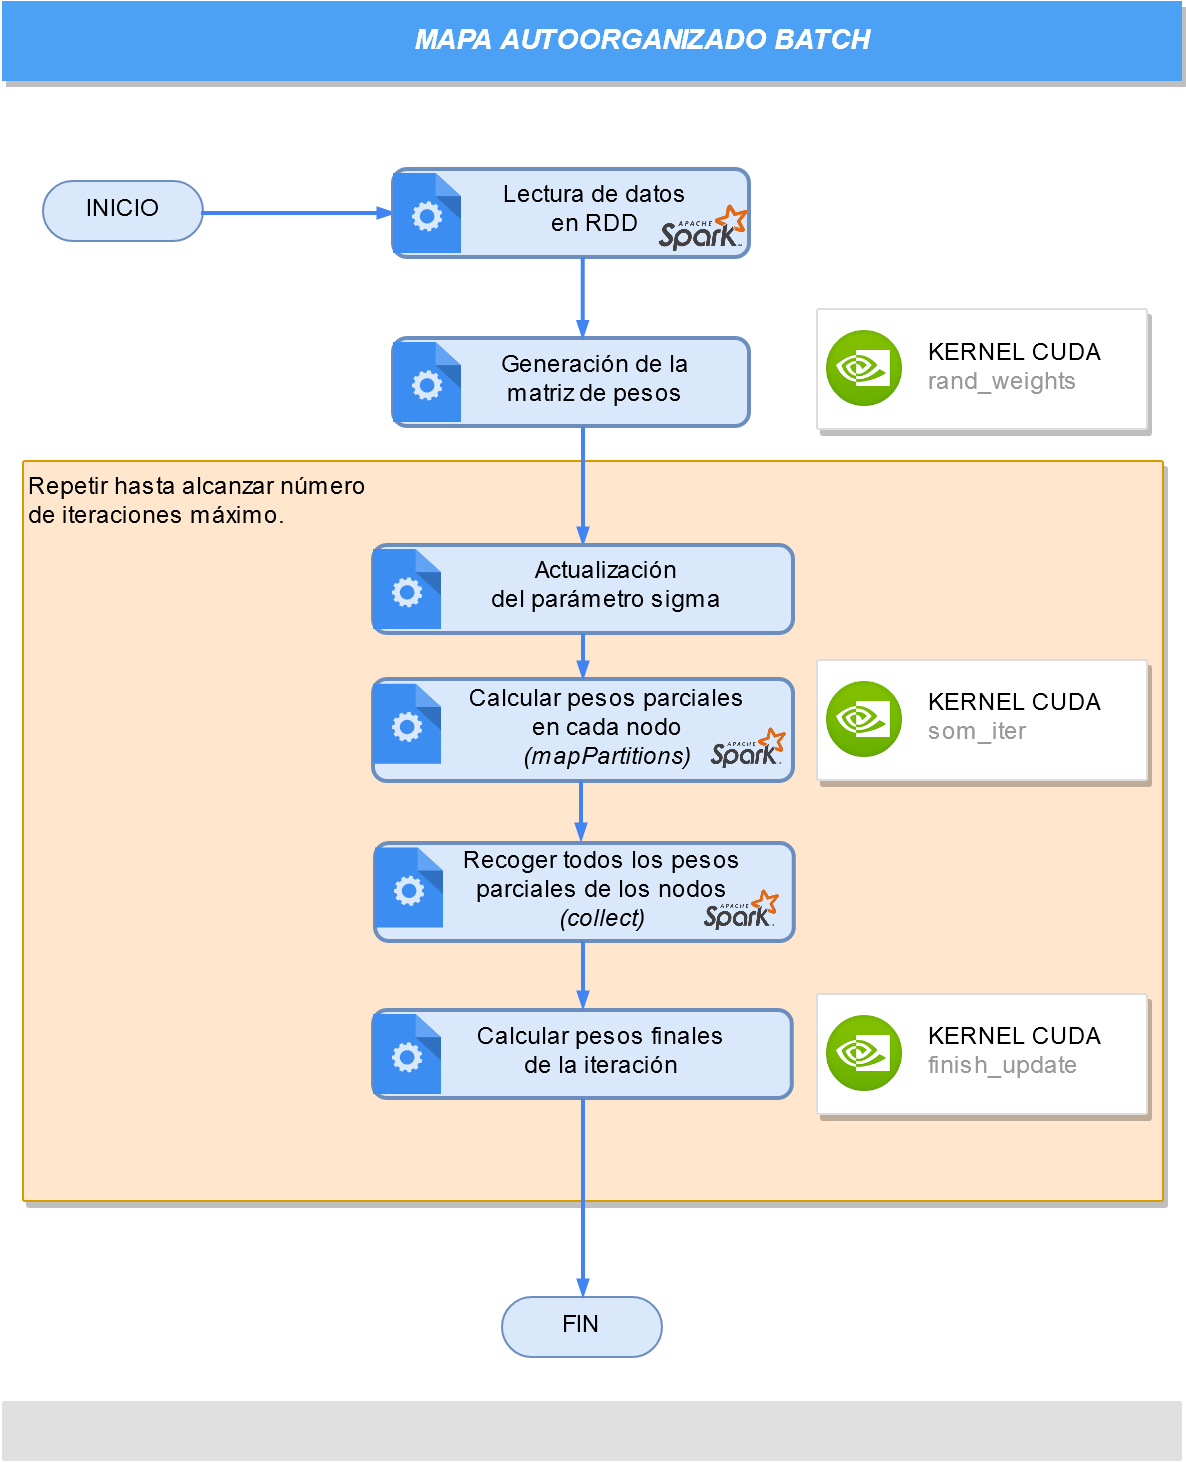
\includegraphics[scale=0.39]{imagenes/flujosparksom.png}
\caption{Diagrama de flujo del mapa auto-organizado desarrollado.}
\label{image:flujosparksom}
\end{figure}

Utilizar \textit{Spark} para implementar este algoritmo nos permite afrontar problemas de tamaños superiores a la capacidad de memoria de nuestro dispositivo, siempre que la memoria necesaria para evaluar una partición del \textit{RDD} quepa en la memoria del dispositivo, como llevar la implementación realizada a un clúster con múltiples nodos, si cada nodo tiene acceso a un dispositivo \textit{CUDA} con todas las dependencias de \textit{software} instaladas.\\


El algoritmo empieza en un único nodo de \textit{Spark} utilizando el primer kernel desarrollado, \textit{rand\_weights}, para inicializar de manera pseudoaleatoria los valores de la estructura de pesos, en función de una semilla proporcionada por el usuario. Con esta estructura ya generada, empieza el proceso iterativo en el que:
\begin{itemize}
    \item 1) Calculamos el parámetro de control $\sigma$ para la iteración en función de las ecuación correspondiente.

$$\sigma(t) = \left\{
\begin{array}{ll}
\sigma_0e^{-\frac{t}{\tau}} & si \;\;t < z\\
\sigma_f & si  \;\; t\geq z
\end{array}
\right.
$$\\
    \item 2) Utilizando la transformación \textit{mapPartitions}, en cada partición del \textit{RDD} se aplica la función \textit{gpu\_work\_iter}, que encapsula el segundo  \textit{kernel} desarrollado, \textit{som\_iter}. Este \textit{kernel} se encarga de evaluar los pesos parciales para cada neurona en función de las muestras asociadas a la partición del \textit{RDD}. Puesto que la actualización de pesos es una división entre una sumatoria de vectores, con cada vector del tamaño de una muestra, y una sumatoria de números reales, el objetivo de cada partición será calcular esos numeradores y denominadores, a los que nos referiremos de ahora en adelante como numeradores y denominadores parciales.
    $$
 W_{i, j} = \frac{\sum_{k=0}^{f} \delta_f(c, [i,j]) \cdot  X(T_k) }{\sum_{k=0}^{f} \delta_f(c, [i,j])}
$$
    \item 3) Para finalizar la iteración, \textit{Spark} reúne mediante \textit{collect} las numeradores y denominadores parciales obtenidos y, usando el último \textit{kernel} implementado, \textit{finish\_update} obtiene los pesos finales de la iteración.\\
\end{itemize}

Este proceso, que consta de 3 fases, es realizado hasta alcanzar el número máximo de iteraciones. Hemos de destacar que todas las particiones han de partir de la mismos pesos en cada iteración para realizar los cálculos. Por ello, al inicio de la iteración, es necesario distribuir la matriz de pesos a cada nodo de \textit{Spark} que realiza esos cálculos y, al final de la iteración, reunir todos los numeradores y denominadores parciales en un único nodo, permitiéndonos obtener los pesos finales de la iteración. \\

Para que \textit{Spark} pueda realizar esa distribución a lo largo de un clúster es necesario que, al final de la iteración, se haga la transferencia de memoria de dispositivo a \textit{host} de los pesos parciales y, al inicio de la iteración, se haga la transferencia de \textit{host} a dispositivo de la pesos de las neuronas correspondientes a esa iteración.\\

\begin{code}
\begin{minted}[fontsize=\footnotesize]{python}

def spark_gpu_batch_som(rdd_data, d, max_iters, rows, cols, smooth_iters=None,
                        sigma_0=10, sigma_f=0.1, tau=400, seed=None, tpb=128):
    """
    :param rdd_data RDD con el conjunto de muestras a evaluar.
    :param d Tamaño de una muestra, dimensión del problema.
    :param max_iters Número de iteraciones a realizar.
    :param rows Número de filas en el mapa de neuronas.
    :param cols Número de columnas en el mapa de neuronas.
    :param smooth_iters Número de iteraciones en las que el parámetro
           sigma decrece siguiendo una función gaussiana. 
    :param sigma_0 Valor de sigma inicial.
    :param sigma_f Valor de sigma tras alcanzar la iteración smooth_iters.
    :param tau Valor de tau para la función gaussiana.
    :param seed Semilla pseudoaleatoria para la generación inicial de pesos.
    :param tpb Número de hebras por bloque para la inicialización de pesos y
           la actualización final de los pesos.
    """
    # 1. Declaramos la estructura de los pesos.
    d_weights = cuda.device_array((rows, cols ,d), np.float32)

    # 1.2 Usamos Numba para generar los pesos de forma pseudoaleatoria.
    rng_states = create_xoroshiro128p_states(rows * cols * d, seed=seed)
    rand_weights[(d_weights.size) // tpb + 1, tpb](rng_states, d_weights)
     
    # 1.3 Traemos los pesos de la memoria de la GPU a la memoria del host.
    weights = d_weights.copy_to_host()

    # 2. Inicio del proceso iterativo
    for t in range(max_iters):
        # 2.a Actualizamos sigma en función de los tau y la iteración.
        if smooth_iters is None or t < max_iters:
            sigma = sigma_0 * math.exp((-t/tau))
        else:
            sigma = sigma_f
            
        sigma_squared = sigma * sigma
        
        # 2.b Cálculos parciales con mapPartitions en cada nodo.
        out = rdd_data.mapPartitions(gpu_work_iter(weights, sigma_squared))
        
        # 2.c En un único nodo calculamos las sumas parciales.
        out = out.collect()
        finish_update[rows*cols//tpb + 1, tpb](weights, np.concatenate(out), 
                                               len(out) // 2)
       
    # 3. Devolvemos los pesos obtenidos
    return weights
\end{minted}
\captionof{listing}{Uso de Spark para entrenar el mapa auto-organizado.}
\label{code:somspark}
\end{code}

\subsection{Representación de la estructura de pesos de las neuronas.}
La estructura que contiene los pesos de las neuronas, que durante la ejecución de los \textit{kernels} se encontrará almacenada en la memoria global del dispositivo, se corresponde a un array tridimensional. El primer eje indica la fila que ocupa la neurona en el mapa, el segundo eje indica la columna que ocupa la neurona en el mapa y el último eje la característica del problema a la que queremos acceder.\\

Mientras que nosotros podemos hacer uso de este sistema de indexación tridimensional gracias a Numba, en realidad, en el dispositivo CUDA se trata de un array unidimensional \textit{row-major}.


\begin{figure}[ht]
\centering
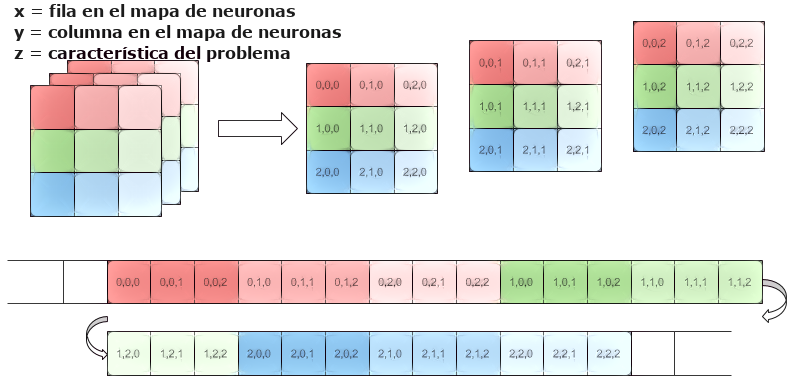
\includegraphics[scale=2.0]{imagenes/row-major.png}
\caption{Representación de un array 3D como un array 1D row-major.}
\label{image:rowmajor}
\end{figure}

\subsection{Kernels implementados.}
\subsubsection{Generación pseudoaleatoria de pesos de neuronas.}
\begin{code}
\begin{minted}[fontsize=\footnotesize]{python}
@cuda.jit
def rand_weights(rng_states, d_weights):
    """
    Kernel para inicializar aleatoriamente la estructura de pesos con 
    valores en el intervalo [0, 1) tomados de una distribución uniforme
    :param rng_states Estados aleatorios.
    :param d_weigths Vector de filas * columnas * d valores que contendrá 
           los pesos asociados a las neuronas.
    """
    # La hebra coge su identificador unidimensional único.
    idx = cuda.grid(1)

    # La hebra calcula en función del su índice 
    # y cocientes y restos de divisiones entereas
    n_rows, n_cols, d = d_weights.shape

    # Cálculo de la fila (eje X).
    row = idx // (n_cols * d)

    # Cálculo de la columna (eje Y).
    col_d = idx % (n_cols * d)
    col = col_d // d
    # Cálculo de la característica (eje Z).
    i = col_d % d
    
    # Sacamos el aleatorio correspondiente.
    if idx < d_weights.size:
        d_weights[row, col, i] = xoroshiro128p_uniform_float32(rng_states, idx)

\end{minted}
\captionof{listing}{Inicialización pseudoaleatoria de los pesos de las neuronas.\\}
\label{code:numbainitweights}
\end{code}

Este proceso (código fuente \ref{code:numbainitweights}) es realizado por el nodo de Spark que controlaría la ejecución del clúster una única vez al inicio del algoritmo, pero utilizando la GPU. \textit{Numba CUDA} nos proporciona herramientas para la generación de valores flotantes en el rango comprendido entre 0 y 1 basadas en el método de Box-Muller. Hemos utilizado esta herramienta para la generación de nuestra matriz de vectores de pesos inicial. Una vez generados, son trasladados de vuelta a la CPU para ser distribuidos a todos los nodos ejecutores de \textit{Spark}. \\

Al lanzar este kernel, se utilizan tantas hebras como números aleatorios (tabla \ref{tab:randkernel}), distribuidos en bloques de un tamaño indicado por el usuario.
\begin{table}[ht]
\begin{tabular}{@{}lll@{}}
\toprule
\textbf{Kernel}        & \textbf{Bloques}                                 & \textbf{Hebras por bloque}                                                                       \\ \midrule
\textbf{rand\_weights} & ($filas$ $\cdot$ $columnas$ $\cdot$ $d$) $//$ $tpb$ + 1 & $tpb$ \\ \bottomrule
\end{tabular}

\textit{\\$d=$ dimensión del problema.\\$tpb=$ hebras por bloque (indicados por el usuario).\\ $//=$ cociente de división entera.}
\caption{Parámetros para el lanzamiento del kernel rand\_weights.}
\label{tab:randkernel}
\end{table}
\newpage
\subsubsection{Cálculo de los numeradores y denominadores parciales.}
\begin{code}
\begin{minted}[fontsize=\footnotesize]{python}
def gpu_work_iter(weights, sigma_squared):
    def _gpu_work(data):
        # 1. Procesamos el dataset
        inp = np.asarray(list(data), dtype=np.float32)
        rows, cols, d = weights.shape
        nneurons = rows * cols
        
        # 2. Pasamos los datos a las memorias del dispositivo
        d_samples = cuda.to_device(inp)
        d_weights = cuda.to_device(weights)
        nums = np.zeros(rows * cols * d, np.float32)
        denums = np.zeros(rows * cols, np.float32)
        d_nums = cuda.to_device(nums)
        d_denums = cuda.to_device(denums)
        
        # 3. Tomamos el número de hebras por bloque
        if nneurons > 1024:
            raise Exception('Número de neuronas superior al límite')
        # Número de hebras necesario para que funcione la reducción.
        tpb = max(64,2**(math.ceil(math.log2(nneurons))))
        # 4. Lanzamos el kernel.
        # Memoria compartida para almacenar una muestra por bloque
        sm_size = 4 * d
        som_iter[N, tpb, 0, sm_size](d_samples, d_weights, d_nums, d_denums,
                                     sigma_squared)
        
        return d_nums.copy_to_host(), d_denums.copy_to_host()
    return _gpu_work
\end{minted}
\captionof{listing}{Función a ejecutar con mapPartitions.\\}
\label{code:somencapsulado}
\end{code}
Una vez obtenidos los pesos iniciales de una iteración, el siguiente paso es utilizar \textit{mapPartitions} para obtener los pesos parciales de cada partición del \textit{RDD}, como veíamos en el código fuente \ref{code:somspark}. La función utilizada en cada partición se denomina \textit{gpu\_som\_iter} y encapsula el lanzamiento del kernel \textit{som\_iter} y las transferencias de memoria entre host y dispositivo en cada iteración.\\

\begin{table}[ht]
\centering
\begin{tabular}{@{}lll@{}}

\toprule
\textbf{Kernel}        & \textbf{Bloques}                                 & \textbf{Hebras por bloque}                                                                       \\ \midrule
\textbf{som\_iter} &   Nº de muestras. & $max(64,2^{techo(\log_2{Nº neuronas})})$ \\ \bottomrule
\end{tabular}
\textit{\\techo=menor número entero mayor o igual que un número real.}
\caption{Parámetros para el lanzamiento del kernel som\_iter.}
\label{tab:iterkernel}
\end{table}

El \textit{kernel som\_iter} es la parte más importante de la implementación del algoritmo y realiza todas las operaciones necesarias para obtener los numeradores y denominadores parciales de la iteración.



\begin{code}
\begin{minted}[fontsize=\footnotesize]{python}
@cuda.jit
def som_iter(d_samples, d_weights, d_nums, d_denums, sigma_squared):
    """
    :param d_samples Conjunto de todas las muestras a evaluar.
    :param d_weigths Vector de filas * columnas * d valores que contendrá 
           los pesos asociados a las neuronas.
    :param d_nums Vector con los numeradores para el cálculo de la fórmula.
    :param d_denums Vector con los denominadores para el cálculo de la fórmula.
    :param sigma_squared Valor de sigma al cuadrado para el cáculo del vecindario.
    """
    nrows, ncols, d = d_weights.shape
    nneurons = nrows * ncols
    
    sample_idx, nueron_idx = cuda.blockIdx.x, cuda.threadIdx.x
    neuron_row, neuron_col = neuron_idx // ncols, neuron_idx % ncols
    blockSize = cuda.blockDim.x
       
    # 0. Declaramos la memoria compartida
    shared_sample = cuda.shared.array(shape=0, dtype=numba.float32)
    shared_distances = cuda.shared.array(shape=1024, dtype=numba.float32)
    shared_idx = cuda.shared.array(shape=1024, dtype=numba.int32)
    
    # 1.a Cada hebra pone una posición de la muestra en memoria compartida.
    # El bucle for permite realizar esto si la dimensión del problema fuese
    # superior al número de neuronas.
    for i in range(d // nneurons + 1):
        i_stride = i * nneurons
        my_pos = i_stride + cuda.threadIdx.x
        # Si la posición que corresponde a la hebra no supera el
        # tamaño de la muestra a cargar.
        if my_pos < d: 
            shared_sample[my_pos] = d_samples[sample_idx, my_pos]
    # Sincronizamos para asegurar que la muestra ha sido cargada.
    cuda.syncthreads()
    
    # 1.b Calculamos las distancias euclídeas que nos corresponden.
    if neuron_idx < nneurons:
        shared_distances[neuron_idx] = 0.0
        for i in range(d):
            i_distance = shared_sample[i] - d_weights[neuron_row, neuron_col, i]
            shared_distances[neuron_idx] += i_distance * i_distance
    # Si hay más hebras que neuronas inicializamos a infinito para la reducción.
    else: 
        shared_distances[neuron_idx] = np.inf
    
    # 1.c Inicializamos el array de índices para la reducción.
    shared_idx[neuron_idx] = neuron_idx
    # Sincronizamos para asegurar los arrays han sido inicializados.
    cuda.syncthreads()    
\end{minted}
\captionof{listing}{Primer fragmento [Cálculo de distancias] de som\_iter.\\}
\label{code:somiter1}
\end{code}

El kernel comienza con la declaración e inicialización de la memoria compartida.\\

En primer lugar, cada hebra contribuye a cargar una característica de la muestra a evaluar por el bloque hasta la muestra ha sido cargada por completo. En segundo lugar, generamos dos arrays adicionales en memoria compartida, que serán utilizados posteriormente para calcular la BMU. Puesto que hemos limitado nuestra implementación a funcionar con un máximo de 1024 neuronas, que es el máximo de hebras por bloque, estos dos arrays serán siempre de esta dimensión. Uno de ellos, que será de \textit{floats} de 32 bits, contendrá las distancias entre la muestra que cargamos en memoria compartida y los pesos de cada neurona del mapa. El segundo, que será de enteros de 32 \textit{bits}, será inicializados con los índices de cada neurona. Para realizar el cálculo de la distancia euclídea, cada hebra calculará su distancia con la neurona que le corresponde y la muestra cargada en memoria compartida. Si hubiese más hebras en el bloque que neuronas en el mapa, el resto de distancias son inicializadas a infinito. \\

Puesto que nuestro siguiente objetivo será encontrar la BMU, es decir, la neurona con menor distancia, no es necesario calcular la raíz cuadrada de la división euclídea, ya que ésta no afecta a la relación de orden. Para encontrar la distancia mínima, utilizamos un algoritmo frecuentemente utilizando en la GPU: \textbf{la reducción}.
\begin{figure}[ht]
\centering
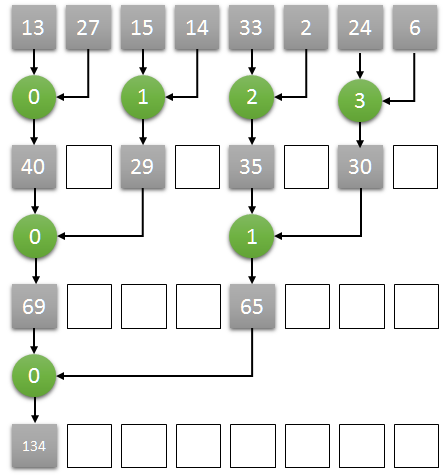
\includegraphics[scale=0.5]{imagenes/parallel_reduce.png}
\caption{Una reducción paralela de una sumatoria.}
\label{image:cudareduction}
\end{figure}

\begin{code}
\begin{minted}[fontsize=\footnotesize]{python}
    # Recorrido de árbol de hojas a la raíz (posición 0)
    if blockSize >= 1024 and neuron_idx < 512:
        if shared_distances[neuron_idx + 512] < shared_distances[neuron_idx]:
            shared_distances[neuron_idx] = shared_distances[neuron_idx + 512]
            shared_idx[neuron_idx] = shared_idx[neuron_idx + 512]
    cuda.syncthreads()
    
    if blockSize >= 512 and neuron_idx < 256:
        if shared_distances[neuron_idx + 256] < shared_distances[neuron_idx]:
            shared_distances[neuron_idx] = shared_distances[neuron_idx + 256]
            shared_idx[neuron_idx] = shared_idx[neuron_idx + 256]
    cuda.syncthreads()
    
    if blockSize >= 256 and neuron_idx < 128:
        if shared_distances[neuron_idx + 128] < shared_distances[neuron_idx]:
            shared_distances[neuron_idx] = shared_distances[neuron_idx + 128]
            shared_idx[neuron_idx] = shared_idx[neuron_idx + 128]
    cuda.syncthreads()
    
    if blockSize >= 128 and neuron_idx < 64:
        if shared_distances[neuron_idx + 64] < shared_distances[neuron_idx]:
            shared_distances[neuron_idx] = shared_distances[neuron_idx + 64]
            shared_idx[neuron_idx] = shared_idx[neuron_idx + 64]
    cuda.syncthreads()
    
    if neuron_idx < 32: # Unroll de warp. No necesitamos sincronizar.
        if shared_distances[neuron_idx + 32] < shared_distances[neuron_idx]:
            shared_distances[neuron_idx] = shared_distances[neuron_idx + 32]
            shared_idx[neuron_idx] = shared_idx[neuron_idx + 32]
        if shared_distances[neuron_idx + 16] < shared_distances[neuron_idx]:
            shared_distances[neuron_idx] = shared_distances[neuron_idx + 16]
            shared_idx[neuron_idx] = shared_idx[neuron_idx + 16]
        if shared_distances[neuron_idx + 8] < shared_distances[neuron_idx]:
            shared_distances[neuron_idx] = shared_distances[neuron_idx + 8]
            shared_idx[neuron_idx] = shared_idx[neuron_idx + 8]
        if shared_distances[neuron_idx + 4] < shared_distances[neuron_idx]:
            shared_distances[neuron_idx] = shared_distances[neuron_idx + 4]
            shared_idx[neuron_idx] = shared_idx[neuron_idx + 4]
        if shared_distances[neuron_idx + 2] < shared_distances[neuron_idx]:
            shared_distances[neuron_idx] = shared_distances[neuron_idx + 2]
            shared_idx[neuron_idx] = shared_idx[neuron_idx + 2]
        if shared_distances[neuron_idx + 1] < shared_distances[neuron_idx]:
            shared_distances[neuron_idx] = shared_distances[neuron_idx + 1]
            shared_idx[neuron_idx] = shared_idx[neuron_idx + 1]
    cuda.syncthreads()
    
    # La mejor neurona se encuentra en la posición 0 del array.
    bmu = shared_idx[0]
    bmu_row, bmu_col = bmu // ncols, bmu % ncols
    cuda.syncthreads()
\end{minted}
\captionof{listing}{Segundo fragmento [Reducción] del kernel som\_iter.\\}
\label{code:somiter2}
\end{code}
  
La reducción puede utilizarse para obtener el resultado de aplicar un operador binario a lo largo de un array, siempre que el operador en cuestión cumpla la propiedad asociativa. En nuestro caso, dicho operador es el mínimo entre dos elementos. Para realizar esta operación de manera eficiente dentro de un bloque, se simula un recorrido hacia arriba sobre un árbol binario balanceado (figura \ref{image:cudareduction}), en el que vamos aplicando la operación sobre los dos hijos y guardando el resultado en el nodo padre, tomando los distancias cargadas en memoria compartida como las hojas y alcanzado el resultado final en la raíz. Por ello, era necesario que el número de hebras por bloque fuese potencia de 2, si teníamos más hebras que neuronas completábamos las distancias con infinito, que actúa como elemento neutro de la operación mínimo, y, añadíamos un array extra con los índices para propagar la posición con el mejor índice mientras hacemos el recorrido. Podemos consultar con más detalle cómo realizar una implementación de una reducción de alto rendimiento en \textit{CUDA} en la referencia bibliográfica \cite{reduction}.\\


Para finalizar el \textit{kernel}, se realiza el cálculo de los numeradores y denominadores parciales. Para ello, cada hebra del bloque se corresponde con una neurona y mide la distancia euclídea que existe entre la posición de la BMU y la posición de la neurona en el mapa. Si esa distancia es menor o igual que el parámetro de control $\sigma^2$, se realiza la suma del vector del numerador con el producto de esa distancia y la muestra guardada en la memoria compartida del bloque y sólo la distancia con el denominador. \\
\begin{code}
\begin{minted}[fontsize=\footnotesize]{python}
# 3. Realizamos la actualización de los pesos.
    if neuron_idx < nneurons:
        dist = (neuron_row - bmu_row) * (neuron_row - bmu_row) + \
               (neuron_col - bmu_col) * (neuron_col - bmu_col)
        # Si estamos dentro del rango de actualización.
        if dist <= sigma_squared:
            hck = math.exp(-dist/(2 * sigma_squared))
            # Guardamos sumatoria del denominador.
            cuda.atomic.add(d_denums, neuron_row * ncols + neuron_col, hck)
            # Guardamos sumatoria del numerador.
            for i in range(d):
                cuda.atomic.add(d_nums, neuron_row*ncols*d + neuron_col*d+i,
                                hck * shared_sample[i])
\end{minted}
\captionof{listing}{Tercer y último fragmento del kernel som\_iter.\\}
\label{code:somiter3}
\end{code}


Puesto que múltiples hebras pueden tener la misma BMU y, por tanto, estar actualizando las mismas posiciones en memoria a la vez se utilizan \textbf{operaciones atómicas}, que evitan las condiciones de carrera que pueda surgir a cambio de una mayor latencia en la operación. Hemos de indicar que, para las operaciones atómicas, necesitamos trabajar con arrays unidimensionales, por lo que hemos de hacer los cálculos de indexación necesarios para acceder a las posiciones de memoria deseadas.

\subsubsection{Cálculo de los pesos finales de la iteración.}
Una vez todos los resultados han sido recopilados en un nodo de \textit{Spark}, lanzamos el \textit{kernel finish\_update}, que realizará la sumatoria de los numeradores parciales y de los denominadores parciales para cada neurona así como la división entre ambos. Si ninguna muestra activó la neurona en cuestión, es decir, la suma de todos sus denominadores parciales es 0, se mantendrán los pesos de la iteración anterior para esa neurona. En caso contrario,  los pesos de la neurona se corresponden con el vector obtenido de la división. Para lanzar este \textit{kernel} se utilizan tantas hebras como neuronas hay en el mapa, divididas en bloque de \textit{tpb} hebras. Cada hebra realiza los cálculos asociados a una neurona.

\begin{table}[ht]
\begin{tabular}{@{}lll@{}}
\toprule
\textbf{Kernel}        & \textbf{Bloques}                                 & \textbf{Hebras por bloque}                                                                       \\ \midrule
\textbf{finish\_update} & (Nº de neuronas // $tpb$ + 1) & $tpb$ \\ \bottomrule
\end{tabular}
\caption{Parámetros para el lanzamiento del kernel finish\_update.}
\label{tab:updatekernel}
\end{table}

\begin{code}
\begin{minted}[fontsize=\footnotesize]{python}
@cuda.jit
def finish_update(d_weights, partials, numParts):
    """
    :param d_weights Array de pesos de neuronas.
    :param partials Array con sumas parciales.
    :param numParts Número de resultados parciales a procesar.
    """
    idx = cuda.grid(1)
    nrows, ncols, d = d_weights.shape
    if idx < nrows * ncols:
        row, col = idx // ncols, col = idx % ncols
        
        # a) Sumamos todos los parciales en el primer array.
        numsize = nrows * ncols * d
        densize = nrows * ncols
        fullsize = numsize + densize
        for i in range(numParts - 1):
            # Suma de numeradores.
            for k in range(d):
                pos = fullsize * i + row * ncols * d + col * d + k
                partials[row * ncols * d + col * d + k] += partials[pos]
            # Suma de denominadores.
            pos = fullsize * i + numsize + row * ncols + col
            partials[numsize + row * ncols + col] += partials[pos]
    
        # b) Si no es 0 el denominador realizamos la división y cambiamos pesos.
        if partials[numsize + row * ncols + col] != 0:
            for k in range(d):
                d_weights[row, col, k] = partials[row*ncols*d + col*d +k] / \
                                         partials[numsize + row * ncols + col]
\end{minted}
\captionof{listing}{Actualización final de la matriz de pesos.\\}
\label{code:ending}
\end{code}

\section{Desarrollo de un modelo de árbol de decisión.}
La implementación del modelo de árbol de decisión se basa en CUDT \cite{cudt}, que a su vez se fundamenta en SPRINT \cite{sprint} y la operación de \textit{scan}.

\subsection{Lista de atributos.}
Una lista de atributos, es una estructura auxiliar, procedente de SPRINT \cite{sprint}, utilizada para representar las clases y los atributos asociados a una muestra. Una lista de atributos tiene una estructura similar a la siguiente tabla:

\begin{table}[ht]
\centering
\begin{tabular}{@{}lll@{}}
\toprule
Valor & Clase & ID Muestra \\ \midrule
2,5   & 0     & 0          \\
4,7   & 0     & 1          \\
0,1   & 1     & 2          \\
1,0   & 1     & 3          \\ \bottomrule
\end{tabular}
\caption{Una lista de atributos sin ordenar.}
\label{tab:ejlistaatributos}
\end{table}

Las columnas de la tabla \ref{tab:ejlistaatributos} son:
\begin{itemize}
    \item \textbf{Valor}, que se corresponde al valor que toma el atributo al que corresponde la tabla en la muestra representada en la fila.
    \item \textbf{Clase}, que se corresponde a la etiqueta de salida asociada a la muestra de la fila.
    \item \textbf{ID Muestra}, que se corresponde al identificador de la muestra. Al principio, se corresponde al número de fila empezando por 0.
\end{itemize}

Una vez esta estructura es generada para cada atributo del problema en cuestión, es ordenada por orden creciente según la columna ``Valor''. En la implementación realizada, se utiliza un array para cada columna.

\subsection{Esquema general del algoritmo implementado.}
\begin{figure}[ht]
\centering
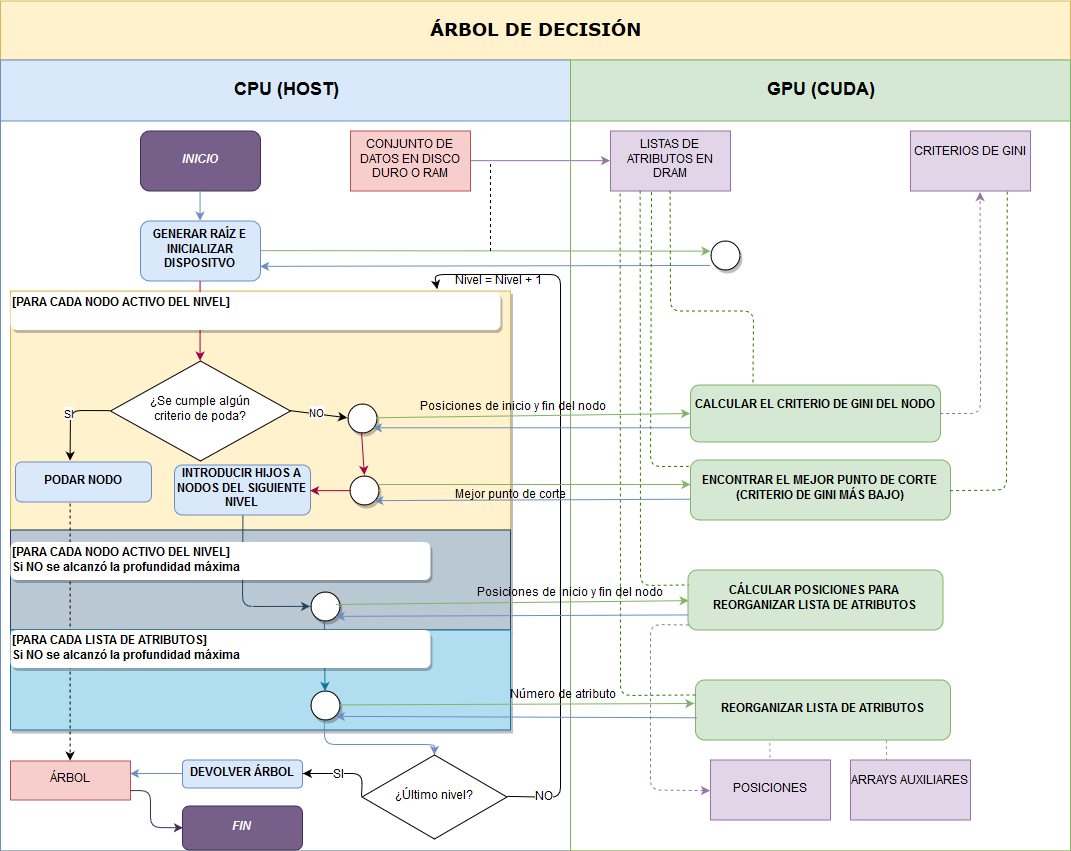
\includegraphics[scale=0.35]{imagenes/esquemadtree.png}
\caption{Diagrama de flujo de la implementación del árbol de decisión.}
\label{img:dtree}
\end{figure}
Al inicio del algoritmo, tras generar las listas de atributos, se genera un nodo raíz que comprende todas las muestras del conjunto. En ese nodo, hemos de encontrar para qué atributo y qué valor realizamos la partición óptima de los datos. Para ello, se consideran todas las listas de atributos y se toma como posible punto de corte el punto medio entre un valor y el siguiente si no se trata del mismo valor. Asociada a cada una de las particiones, se calcula el criterio de Gini. Una vez realizados todos los cálculos, tomamos como punto de corte aquella que menor criterio de Gini nos de. Utilizando ese punto de corte, generamos dos nuevos nodos para la siguiente iteración, uno que contiene todos los puntos menores o iguales que dicho punto de corte y otro con los mayores. Además, dicho punto es el que utilizamos para generar nuestro nodo de decisión en el árbol entrenado.  Este proceso se repite hasta que no quedan nodos por evaluar. Un nodo no ha de ser evaluado si:\\

\begin{itemize}
    \item a) Todos los elementos del nodo pertenecen a la misma clase. En ese caso, en vez de un nodo de decisión, generamos un nodo terminal con la clase correspondiente.
    \item b) Se ha especificado un criterio de profundidad máxima y dicha profundidad ha sido alcanzada. En ese caso, generamos un nodo terminal con la clase más representativa del nodo.
    \item c) Se ha especificado un límite para el número de elementos mínimo que puede contener y ha sido alcanzado. En ese caso, generamos un nodo terminal de manera similar al caso anterior.
\end{itemize}



\subsection{La operación de scan.}
Una de las claves del uso de la lista de atributos, es que, para los problemas de \textbf{clasificación binaria}, que son los únicos que nuestro modelo es capaz de resolver, si codificamos una clase como $0$ (a partir de ahora llamada \textit{clase negativa}) y otra como $1$ (\textit{clase positiva}) si realizamos una suma acumulada sobre el subconjunto de filas de un nodo de la columna ``Clase'' podríamos tener control de cuántos elementos hay en cada clase tanto para todas las particiones. Para realizar la suma acumulada existe una primitiva ampliamente utilizada en el mundo de la GPU denominada \textit{scan}.\\

El \textit{scan} \cite{scan}, suma acumulada o suma prefija, es una operación que utiliza un operador binario, $\oplus$, que cumpla la propiedad asociativa y utilizada sobre un \textit{array} de $n$ elementos. Existen dos formas de realizar el \textit{scan}: inclusivo y exclusivo. El scan inclusivo empieza con el primer elemento del array y va a realizando una suma acumulada. El \textit{scan} exclusivo empieza con el elemento neutro de la operación y realiza una suma acumulada de todos los elementos hasta el penúltimo. En la implementación realizada, hemos utilizado el \textit{scan inclusivo}. Por tanto, para los propósitos de este documento, cada vez que hablemos de \textit{scan}, nos estaremos refiriendo al \textit{scan inclusivo}, que al aplicarla sobre un array, nos devuelve lo siguiente:\\
$$scan([a_0, a_1, a_2, ..., a_{n-1}]) = [ a_0, (a_0 \oplus a_1), (a_0 \oplus a_1 \oplus a_2), ..., (a_0 \oplus a_1 \oplus a_2 \oplus ... \oplus a_{n})]$$

La implementación realizada utilizada operaciones directas sobre \textit{warps}, permitiendo que una ejecución más rápida al realizar todas las operaciones directamente sobre los registros del multiprocesador. De manera más específica el procedimiento realizado es el siguiente.\\

\begin{itemize}
    \item \textbf{1.} Se lanza un kernel con una estructura con un número de hebras por bloque predeterminado por el usuario y el mínimo número de bloques para procesar todo el array.\\
    \item \textbf{2.} El objetivo de cada bloque es calcular su \textit{scan} local.
    \item \textbf{2.1} En primer lugar, cada uno de los \textit{warps} del bloque calcula su \textit{scan} local y lo almacena en un array. La operación utilizada para manejar los \textit{warps} es \textbf{shfl\_up\_sync}. Esta operación nos permite realizar una copia y desplazamiento hacia la derecha en el warp en función de una máscara, un valor y un desplazamiento. La máscara nos permite es un conjunto de 32 bits que nos permite indicar cuáles de las 32 hebras han de ser usadas. Para nuestra operación, la máscara está activa para todos las hebras. El valor indica qué valores vamos a utilizar para realizar la operación y ese valor será devuelto en caso de salirnos del rango del warp. Por último, el desplazamiento nos sirve para calcular cuántas posiciones nos hemos de desplazar hacia la derecha. Por ello, empezamos con un desplazamiento de 1 y vamos ampliando siguiendo las potencias binarias inferiores a 32. Para que los resultados ya calculados no sean modificados, nos aseguramos de trabajar sólo con las hebras dentro del warp con índice superior o igual al desplazamiento. Así, al tomar el desplazamiento 1, todos los elementos se suman a su anterior y el primero se mantiene constante. Al tomar el desplazamiento 2, sólo tenemos qué realizar la suma del que había dos posiciones antes, y así, sucesivamente, hasta llegar al último valor. Los últimos valores de cada \textit{scan} local serán guardados en un array en memoria compartida.

    \item \textbf{2.2} Una vez las sumas locales de los warps han sido realizadas, hemos de añadir la suma acumulada obtenida en los \textit{warps} previos para obtener el resultado final del bloque. Para ello, se realiza un \textit{scan} de los \textit{warps} previos, obteniendo el array con las sumas acumuladas previas y estas son aplicadas a los elementos del array correspondientes.\\

    \item \textbf{3} Una vez tenemos el \textit{scan} de cada bloque, hemos de realizar un procedimiento similar para llevar el \textit{scan} local del bloque a todo el array. Esto ha sido realizado, o bien mediante sumas atómicas en el mismo \textit{kernel}, que son más lentas que las operaciones normales, o bien combinando el trabajo con otros \textit{kernels} que tenían que ser lanzados de forma independiente.

\end{itemize}



\subsection{Cálculo del criterio de Gini.}
Dado que sólo vamos a calcular el criterio de Gini para problemas de clasificación binaria hemos simplificado el mismo para ahorrarnos algunas operaciones a la hora de realizar el cálculo:

$$CRITERIO(A,v) = \frac{|i: A_i \leq v|}{N} \cdot GINI(|i: A_i \leq v|) + \frac{|i: A_i > v|}{N} \cdot GINI(|i: A_i > v|)$$

$$GINI(D) = 1 - \frac{T_D^2}{N_D^2} - \frac{F_D^2}{N_D^2}$$

Siendo $N_D$ el total de las muestras en el nodo $D$, $T_D$ el total de muestras pertenecientes a la clase positiva y $F_D$ el total de muestras pertenencientes a la clase negativa. Tenemos que:

$$F_D = N_D - T_D$$
Sustituyendo obtenemos que:

$$GINI(D) = \frac{N_D^2-T_D^2- (N_D - T_D)^2}{N_D^2} = \frac{N_D^2 - T_D^2 - (N_D^2+T_D^2 - 2 N_D T_D)}{N_D^2}$$
$$GINI(D) = \frac{-2T_D^2 + 2N_DT_D}{N_D^2} = 2 \frac{T_D(N_D-T_d)}{N_D^2}$$

$$CRITERIO = \frac{N_\leq}{N}\frac{2T_\leq(N_\leq - T_\leq)}{N_\leq^2} + \frac{N_>}{N}\frac{2T_>(N_> - T_>)}{N_>^2}$$
$$CRITERIO = \frac{2}{N}\Big(\frac{T_\leq(N_\leq - T_\leq)}{N_{\leq}} + \frac{T_>(N_> - T_>)}{N_>}\Big)$$

Puesto que además, no es de nuestro interés el valor específico sino obtener el valor óptimo, podemos ahorrarnos la multiplicación por $\frac{2}{N}$. Así pues, calculamos el criterio de la siguiente manera:

$$CRITERIO' = \Big(\frac{T_\leq(N_\leq - T_\leq)}{N_{\leq}} + \frac{T_>(N_> - T_>)}{N_>}\Big)$$

El valor de $CRITERIO'$ oscilará entre 0 y $\frac{N}{2}$ y buscaremos siempre obtener el mínimo valor para este criterio. Dicha búsqueda se realizará de manera similar a la realizada para el modelo anterior con una reducción para encontrar el índice mínimo en cada nodo.

\subsection{Reorganización de la listas de atributos.}
Para finalizar la evaluación de los nodos de un nivel podemos volver a aprovechar la operación de \textit{scan} para reorganizar el orden de los elementos de la lista de atributos sin necesidad de ejecutar ningún algoritmo de ordenación.\\

 Una vez se ha seleccionado la combinación de mejor lista de atributos para un nodo y su punto de corte, puesto que esta lista ya estaba ordenada, todos los elementos hasta el punto de corte pertenecen al nodo hijo izquierdo y los posteriores al nodo hijo derecho. Además, puesto que tenemos en la lista de atributos el campo ``ID Muestra'', podemos generar fácilmente un array de booleanos donde cada elemento indica si la muestra con el ID asociado a su posición.\\

 Si aplicamos la operación de \textit{scan} sobre este array auxiliar, la suma acumulada en cada posición nos indica el número de elementos que pertenecen al nodo hijo codificado con la etiqueta positiva. Por lo que, partiendo de que previamente estaban ordenados podemos hacer la subdivisión y mantener el orden teniendo en cuenta que:\\

 \begin{itemize}
    \item 1. Si el elemento en cuestión pertenece al nodo hijo izquierda (codificado como positivo en el array auxiliar), su nueva posición en la lista de atributos sería la suma acumulada obtenida en el array auxiliar menos uno (para que el primer índice sea el 0).
    \item 2. En caso contrario, la nueva posición es el número total de elementos en el nodo hijo izquierda (para que ambos queden separados) más la diferencia de ese total de elementos del nodo hijo izquierda con la suma acumulada del array auxiliar (que nos indicaría cuántos elementos de la clase negativa llevamos hasta el momento) menos uno (porque la indexación empieza en 0).
 \end{itemize}

\subsection{Representación del árbol.}
Debido a la necesidad de intercomunicación constante entre GPU y CPU el árbol ha sido directamente almacenado en la memoria de la segunda. La representación utilizada para el árbol es una lista de diccionarios de tuplas. En primer lugar, la lista tendrá tantos diccionarios como niveles de profundidad tenga el árbol, siendo el nivel 0 la raíz. El diccionario tendrá como clave de entrada un valor numérico, que se corresponderá a la posición que ocuparía el nodo si recorremos el nivel de izquierda a derecha y no se hubiese podado ningún elemento. De esta manera, si nos encontramos ante un nodo de decisión, sus hijos se encontrarían en el diccionario de la siguiente posición de la lista y sus índices de acceso serían el doble del índice de acceso de su padre o el doble del índice de acceso de su padre más 1, dependiendo de a cuál de los dos hijos queramos acceder. Por último, la descripción que se encuentra en en el diccionario para una clave de acceso es una tupla. Dicha tupla indica si el nodo es decisión o terminal. En el caso de ser un nodo de decisión, dispone de campos para el atributo y su valor de corte. En el caso de ser un nodo terminal, dispone de un campo que indica la clase con la que etiquetar la muestra.\\

\subsection{Uso de Spark.}
Este modelo, al requerir la evaluación independiente de múltiples nodos, como podremos comprobar posteriormente, no escala bien con la generación de árboles profundos o completos. Es por eso que, a la hora de integrar \textit{Spark} en la solución, en vez de generar un único árbol, vamos a generar un \textit{random forest}, es decir, vamos a subdividir la muestras de entrenamiento aleatoriamente de tal manera que cada partición de \textit{Spark} entrenará un árbol y, una vez los árboles han sido entrenados, una muestra a clasificar será evaluada por todos los árboles. La clase de la muestra se corresponderá a la clase que ha sido seleccionada en el mayor número de árboles. \\

Esta solución nos permite, por un lado, reducir problemas de sobreajuste, y, por otro, conseguir precisiones competentes sin necesidad de generar árboles completos u otros sistemas de poda más complejos y evitar los problemas de sincronización y comunicación que generaría el entrenamiento de un único árbol como que todos los nodos de \textit{Spark} tendrían que tener una copia de las listas de atributos y, al terminar cada nivel de profundidad debería de plantearse una estrategia para reordenar las listas de atributos y volver a distribuir los cambios a todos los nodos.


%!TEX root = ../proyecto.tex
\chapter{Desarrollo de pruebas y análisis de resultados.}
\section{Entorno de pruebas.}
Para el desarrollo de las pruebas, mi ordenador personal ha sido utilizado. Las especificaciones ténicas relevantes del mismo son:

\begin{itemize}
\item \textbf{GPU}: \underline{Zotac GeForce GTX 1060 AMP! Edition.}
\end{itemize}

% Please add the following required packages to your document preamble:
% \usepackage{booktabs}
% \usepackage{longtable}
% Note: It may be necessary to compile the document several times to get a multi-page table to line up properly
\begin{longtable}{@{}lc@{}}
\toprule
\multicolumn{1}{c}{\textbf{Características}}     & \textbf{Valor}           \\* \midrule
\endfirsthead
%
\endhead
%
\bottomrule
\endfoot
%
\endlastfoot
%
\textbf{Núcleos CUDA}                            & 1290                     \\
\textbf{Frecuencia del procesador}               & 1771 MHz                 \\
\textbf{Frecuencia de la memoria}                & 4004 Mhz                 \\
\textbf{Memoria global total}                    & 6 GB DDR5                \\
\textbf{Bus de memoria}                          & 192-bit                  \\
\textbf{Compute Capability}                      & 6.1                      \\
\textbf{Número de hebras por bloque}             & 1024                     \\
\textbf{Dimensión máxima del bloque (x, y, z)}   & 1024, 1024, 64           \\
\textbf{Dimensión máxima del ``grid'' (x, y, z)} & 2147483647, 65535, 65535 \\
\textbf{Número de registros por bloque}          & 65536                    \\
\textbf{Memoria compartida por bloque}           & 49152 KB                 \\
\textbf{Número de multiprocesadores}             & 10                       \\
\textbf{Modelo de driver CUDA}                   & WDDM                     \\
\textbf{Versión del driver CUDA}                 & 417.35                   \\
\textbf{Versión del SDK CUDA}                    & 10.0                     \\* \bottomrule
\caption{Características de la GPU NVIDIA GeForce GTX 1060 6 GB}
\label{tab:esptec}\\
\end{longtable}

\begin{itemize}
	\item \textbf{Placa Base:} MSI B450M Bazooka.
	\item \textbf{Sistema Operativo:} Windows 10 Home 64 bits.
	\item \textbf{CPU:} AMD Ryzen 5 2600X.
	\item \textbf{RAM:} Kingston HyperX Fury Black DDR4 2400 MHz PC4-19200 8GB CL15.
\end{itemize}
\section{Conjuntos de datos utilizados.}

Durante la fase de desarrollo del mapa auto-organizado hemos utilizado el conjunto de datos de las \textbf{caras de Olivetti}, creado por \textit{AT\&T Laboratories Cambridge} y descargada a través del paquete de Python \textit{scikit-learn} \cite{olivetti}. Dicho conjunto de imágenes consiste en 400 imágenes de 40 sujetos en escala de grises. Cada muestra son los valores de intensidad de cada píxel con un valor normalizado entre 0 y 1. Además, se proporciona una etiqueta que indica a qué sujeto pertenece cada imagen, pero para los propósitos de nuestro modelo de aprendizaje no supervisado la misma no será utilizada. Las imágenes están en una versión cuadrada de 64x64 píxeles dándonos un total de 4096 valores de intensidad por muestra. \\


Para evaluar el rendimiento de ambos modelos para conjuntos de \textit{Big Data} hemos utilizado \textbf{SUSY} \cite{susy}. Este conjunto de datos contiene 5 millones de muestras con 18 atributos, que se generó a partir de un experimento de física en el que también se intenta diferenciar un proceso que genera partículas supersimétricas (\textit{signal}) de otro proceso que no las genera (\textit{background}). En el caso del mapa auto-organizado, la clase de salida es ignorada. De manera similar al anterior, los datos del conjunto fueron generados a partir de simulaciones de Monte Carlo.


\section{Experimentos para evaluar el mapa auto-organizado.}
\subsection{Verificación de la implementación del modelo.}
En el caso del mapa auto-organizado, tanto la versión como para CPU como para GPU ejecutan el mismo algoritmo, por lo que las métricas de interés durante las ejecuciones realizadas son el tiempo de ejecución y la ganancia. En primer lugar, durante la fase de desarrollo usamos el conjunto de las caras de \textit{Olivetti}, que nos permitió comprobar de manera empírica y visual que los resultados obtenidos por el algoritmo son son correctos. En caso de funcionar correctamente, obtendríamos un conjunto de imágenes con la misma dimensión del mapa de neuronas, que son o se parecen a algunas de las caras de los sujetos, y donde las imágenes más parecidas se encuentran próximas las unas con las otras. \\

Para este experimento, generamos un mapa de 5 filas y 6 columnas, y, ejecutamos el algoritmo durante 50 iteraciones, con 25 para la primera fase y otras 25 para la segunda fase y con los parámetros de control $\sigma_0, \sigma_f$ y $\tau$ a 3, 0,1 y 50, respectivamente. El \textit{RDD} de \textit{Spark} que contiene las muestras de entrada es configurado para utilizar 10 particiones. Mientras que las versiones para CPU y GPU hacen exactamente lo mismo, utilizan métodos distintos para la generación de los pesos aleatorios iniciales. Por ello, para este experimento de verificación, tomamos también las dos medidas de calidad del mapa auto-organizado consideradas: el error de cuantificación y el error topográfico.\\

\begin{figure}[ht]
\centering
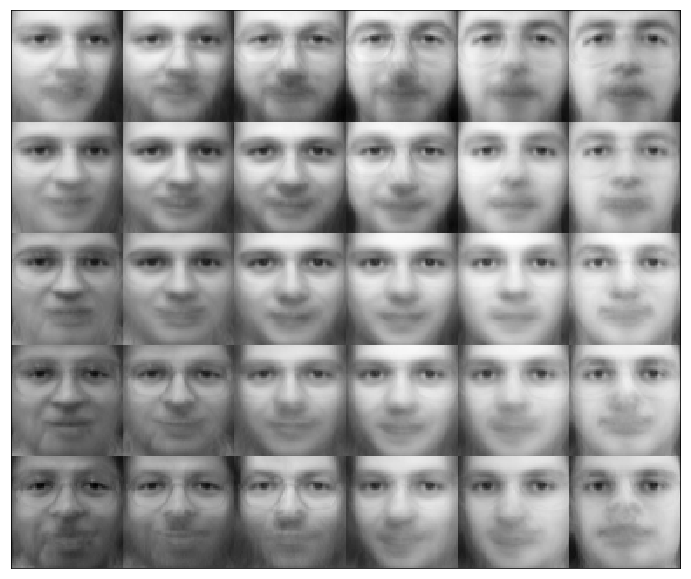
\includegraphics[scale=0.3]{imagenes/facescpu.png}
\caption{Imagen obtenida en el experimento para CPU del mapa auto-organizado.}
\label{img:somcpu}
\end{figure}

\begin{figure}[ht]
\centering
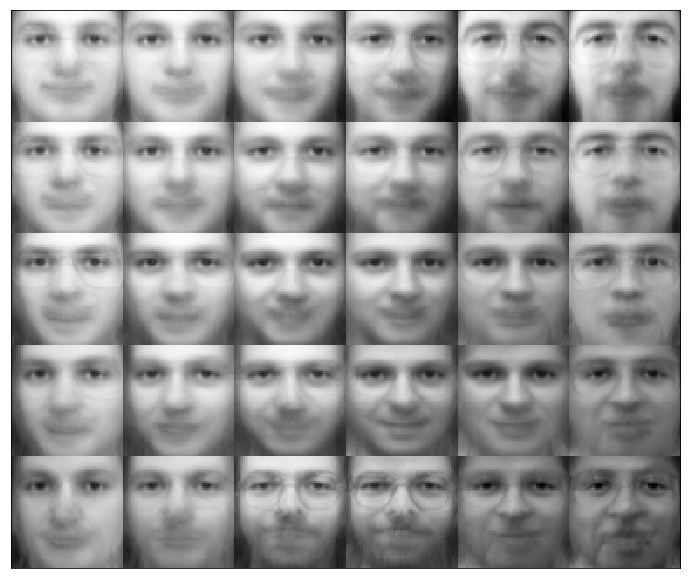
\includegraphics[scale=0.3]{imagenes/facesgpu.png}
\caption{Imagen obtenida en el experimento para GPU del mapa auto-organizado.}
\label{img:somgpu}
\end{figure}

En la figura \ref{img:somcpu}, podemos observar los resultados obtenidos para la ejecución de este algoritmo sobre CPU. En ella, podemos observar que, personas con piel de color más oscuro se agrupan en la esquina superior izquierda, o que, en la fila inferior nos encontramos ante imágenes de la misma persona, donde en las 2 primeras imágenes el sujeto está mirando de lado y, en las siguientes, parece llevar gafas puestas, entre otros detalles. En este ejemplo, obtenemos un error de cuantificación de 6,57 y un error topográfico de 0,0325, tardando un total de 203,09 segundos en su ejecución.\\

En la figura \ref{img:somgpu}, podemos observar los resultados obtenidos para la ejecución de este algoritmo sobre nuestro dispositivo \textit{CUDA}. En ella, podemos observar como, personas que están claramente sonriendo se encuentran en la parte derecha de la penúltima fila, o en la esquina superior derecha, encontramos imágenes del mismo sujeto con gafas puestas. Para este ejemplo, obtenemos un error de cuantificación de 6,56 y un error topográfico de 0,0125, tardando un total de 281,01 segundos en su ejecución.\\
	
En este pequeño experimento, hemos podido comprobar visualmente que ambas implementaciones funcionan correctamente y proporcionan resultados similares, excepto en el tiempo de ejecución, y gran parte de los errores de implementación fueron detectados gracias a este experimento. El hecho de que la versión para GPU tarde más que la versión para CPU a que en cada una de las 10 particiones del \textit{RDD} se evalúan tan sólo 40 muestras y, nuestro algoritmo, en cada iteración y para cada partición, ha de realizar transferencias de memoria entre host y dispositivo, añadiendo un \textit{overhead}. Dado este número bajo de muestras, estamos invirtiendo más tiempo en realizar esas transferencias y lanzar los \textit{kernels} que en los pocos cálculos necesarios. Conforme el número de muestras sea mayor, como veremos en el siguiente experimento, iremos obteniendo mejores resultados con la GPU. 

\subsection{Uso del modelo sobre un conjunto de datos grandes dimensiones.}
Posteriormente, para evaluar la capacidad del algoritmo ante un conjunto de mayores dimensiones, utilizamos SUSY. Para este experimento, ignoramos las etiquetas de salida y utilizamos un mapa de neuronas de 8 filas y 7 columnas con los parámetros de control $\tau$ a 10, $\sigma_0$ a 4, $\sigma_f$ a 0,1. El algoritmo lo ejecutamos durante 10 iteraciones (5 cada fase) y realizamos 4 repeticiones del experimento para tomar una medida de tiempo promedio, con el fin de obtener resultados más fiables que realizando una única ejecución. En este experimento, nos centramos en evaluar como varía el tiempo de ejecución de nuestra implementación y la ganancia conseguida según vamos aumentando el número de muestras totales a evaluar. Nuestro RDD tendrá 10 particiones e iremos variando la cantidad de muestras totales de SUSY que vamos a procesar.

\begin{table}[ht]
\begin{tabular}{@{}l|c|c|c@{}}
\textit{\textbf{Nº de Muestras}} & \multicolumn{1}{l|}{\textit{\textbf{Tiempo CPU (s)}}} & \multicolumn{1}{l|}{\textit{\textbf{Tiempo GPU (s)}}} & \multicolumn{1}{l}{\textit{\textbf{Ganancia}}} \\ \midrule
\textit{\textbf{500000}}         & 231,09                                                & 56,99                                               & 4,06                                          \\
\textit{\textbf{1000000}}        & 426,19                                                & 58,74                                               & 7,26                                           \\
\textit{\textbf{1500000}}        & 618,29                                                & 61,41                                               & 10,07                                           \\
\textit{\textbf{2000000}}        & 822,55                                                & 62,73                                               & 13,11                                           \\
\textit{\textbf{2500000}}        & 1017,45                                               & 66,22                                               & 15,36                                           \\
\textit{\textbf{3000000}}        & 1212,12                                               & 67,75                                               & 17,89                                           \\
\textit{\textbf{3500000}}        & 1398,09                                               & 67,14                                               & 20,83                                           \\
\textit{\textbf{4000000}}        & 1616,68                                               & 67,63                                               & 23,90                                           \\
\textit{\textbf{4500000}}        & 1788,50                                               & 68,45                                               & 26,13                                           \\
\textit{\textbf{5000000}}        & 1992,61                                               & 72,30                                               & 26,99                                          
\end{tabular}
\caption{Tiempos promedios de ejecución y ganancias para el experimento del mapa auto-organizado sobre SUSY.}
\label{tab:susysom}
\end{table}

En la tabla \ref{tab:susysom}, vemos las diferencias entre los tiempos promedios de 4 ejecuciones para CPU y 4 ejecuciones para GPU según los percentiles de muestras propuestos para el experimento. La evolución de los tiempos de ejecución para la GPU oscila en un pequeño intervalo entre los 60-70 segundos (1 minuto). Sin embargo, la evolución de los tiempos para la CPU oscila entre los 231 segundos (casi 4 minutos) y 1992 segundos (33 minutos) por ejecución.  Para una mejor visualización de estos resultados, planteamos la gráfica de la figura \ref{img:somsusy}, en la que combinamos las gráficas de líneas para la evolución de los tiempos promedios con las ganancias obtenidas en una gráfico de barras. \\

\begin{figure}[ht]
\centering
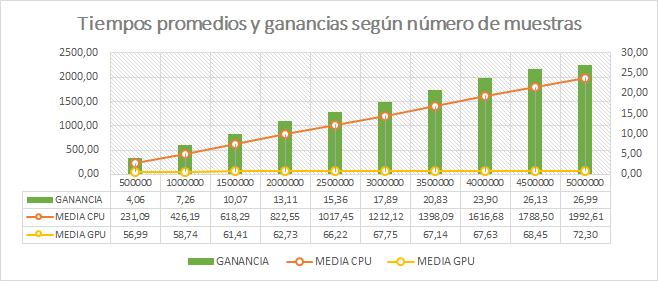
\includegraphics[scale=0.7]{imagenes/susysom.png}
\caption{Gráfica con tiempos promedios y ganancias para SUSY.}
\label{img:somsusy}
\end{figure}

En la gráfica planteada vemos de manera clara cómo, al aumentar el número de muestras, la implementación basada en \textit{CUDA} y \textit{Spark} es considerablemente más rápida que su homóloga para CPU. En el ejemplo más pequeño planteando, es decir, evaluar medio millón de muestras, en el que cada una de las 10 particiones del \textit{RDD} evalúa 50000 muestras, la versión para CUDA es 4 veces más rápida que su homóloga para CPU. En el ejemplo más grande propuesto, es decir, evaluar 5 millones de muestras, el uso de CUDA nos ofrece un tiempo de ejecución casi 27 veces más rápido que la CPU.


\subsection{Resultados de Nsight sobre la versión final del algoritmo.}
Por último, analizamos en profundidad simulamos el entrenamiento del SOM durante una iteración con un ejemplo completamente aleatorio. El total de muestras a evaluar es de 1 millón, divididas en 10 particiones de 100000 muestras. El mapa de neuronas objetivo es de 10 filas por 10 columnas y la dimensión del problema a resolver es de 18 características. En la tabla \ref{tab:profsomkernels}, vemos los tiempos de ejecución de los \textit{kernels} en este experimento.\\

\begin{table}[ht]
\begin{tabular}{@{}|lc|cccc|@{}}
\toprule
                                 & \multicolumn{1}{l|}{}                               & \multicolumn{4}{c|}{\textit{\textbf{Tiempo}}}                                                                                         \\
\textit{\textbf{Kernel}}         & \multicolumn{1}{l|}{\textit{\textbf{Nº usos}}} & \textit{\textbf{mínimo}} & \textit{\textbf{medio}}           & \textit{\textbf{máximo}}          & \textit{\textbf{total}}            \\ \midrule
\textit{\textbf{rand\_weights}}  & 1                                                   & $6,62 \; \mu s$             & $6,62 \; \mu s$                      & $6,62 \;\mu s$                      & $6,62 \;\mu s$                       \\
\textit{\textbf{som\_iter}}      & 10                                                  & $1,61 \; ms$                & $1,835 \; ms$                        & $2,17 \;ms$                         & $18,35 \;ms$                         \\
\textit{\textbf{finish\_update}} & 1                                                   & $37,38 \; \mu s$            & \multicolumn{1}{l}{$37,38\; \mu s$} & \multicolumn{1}{l}{$37,38 \;\mu s$} & \multicolumn{1}{l|}{$37,38 \;\mu s$} \\ \bottomrule
\end{tabular}
\caption{Tiempos de ejecución de los kernels en el experimento de profiling}
\label{tab:profsomkernels}
\end{table}

Como cabía esperar, la mayor parte del tiempo se corresponde a la ejecución del \textit{kernel som\_iter}, que tarda un total de $18,35 \; ms$. El kernel \textit{rand\_weigths} es el más rápido de todos y, aun así, es sólo invocado una vez en el algoritmo, independientemente del número de iteraciones, por lo que no tiene sentido centrarse en optimizarlo mientras se puedan hacer otras mejoras. El kernel \textit{finish\_update}, que será llamado tantas veces como iteraciones se realicen en el algoritmo ocupan el puesto intermedio, siendo 49 veces más rápido que una llamada al \textit{kernel som\_iter}. Además, el \textit{kernel som\_iter}, siempre será llamado las mismas veces que \textit{finish\_update} multiplicado por el número de particiones del \textit{RDD} por lo que, a ser posible, hemos de centrarnos en mejorar este \textit{kernel}.\\

\begin{figure}[ht]
\centering
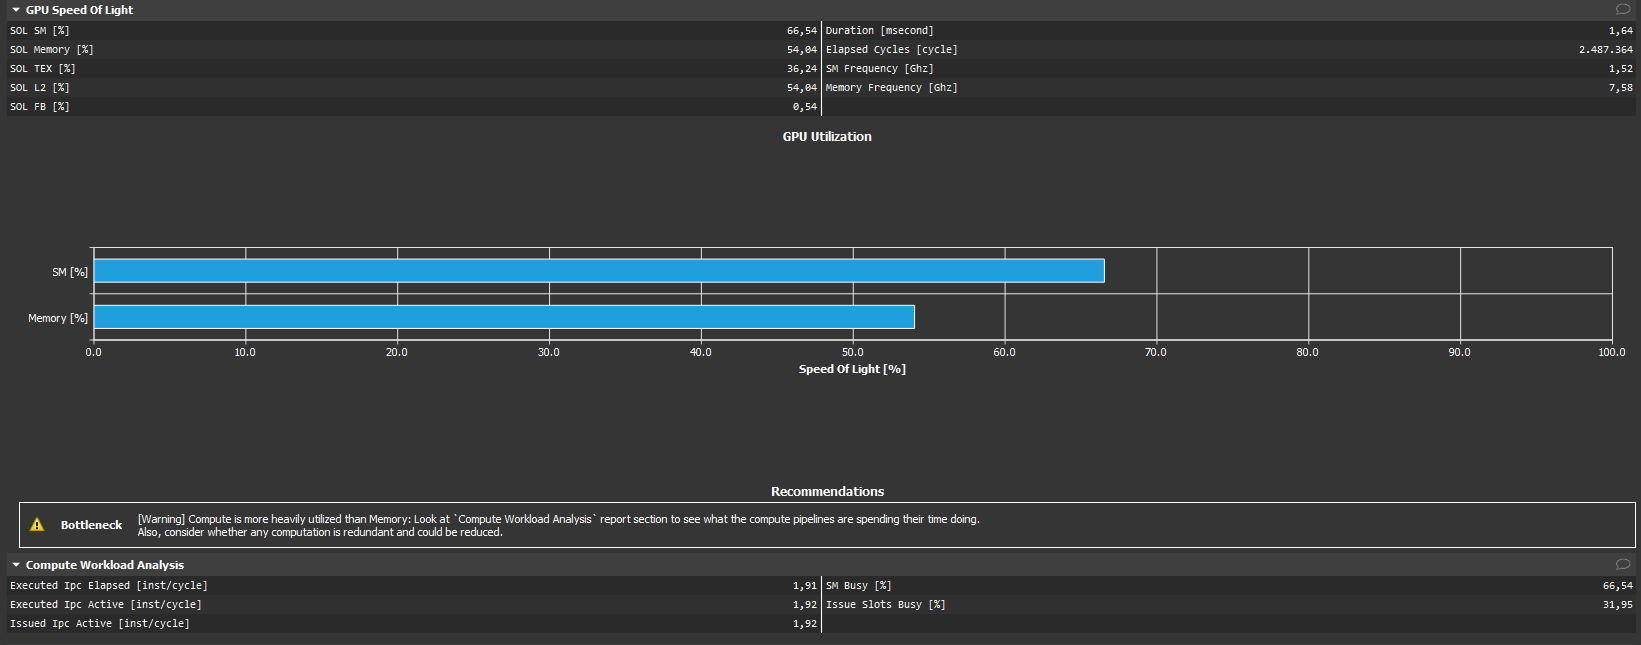
\includegraphics[scale=0.3]{imagenes/som_sol.png}
\caption{Speed of Light del kernel evaluado.}
\label{img:sol}
\end{figure}

Un análisis más profundo del \textit{kernel som\_iter} con el profiler nos revela que, el cuello de botella ,se debe a los cálculos realizados (figura \ref{img:sol}). La medida \textit{``Speed Of Light (SOL)''} nos indica lo cerca que estamos de alcanzar el rendimiento teórico máximo de unidades de \textit{hardware} durante la utilización del dispositivo CUDA en el \textit{kernel}. Podemos observar que, en nuestro caso, estamos aprovechando un 66,54 \% de la capacidad máxima de computación de nuestra GTX 1060.\\

\begin{figure}[ht]
\centering
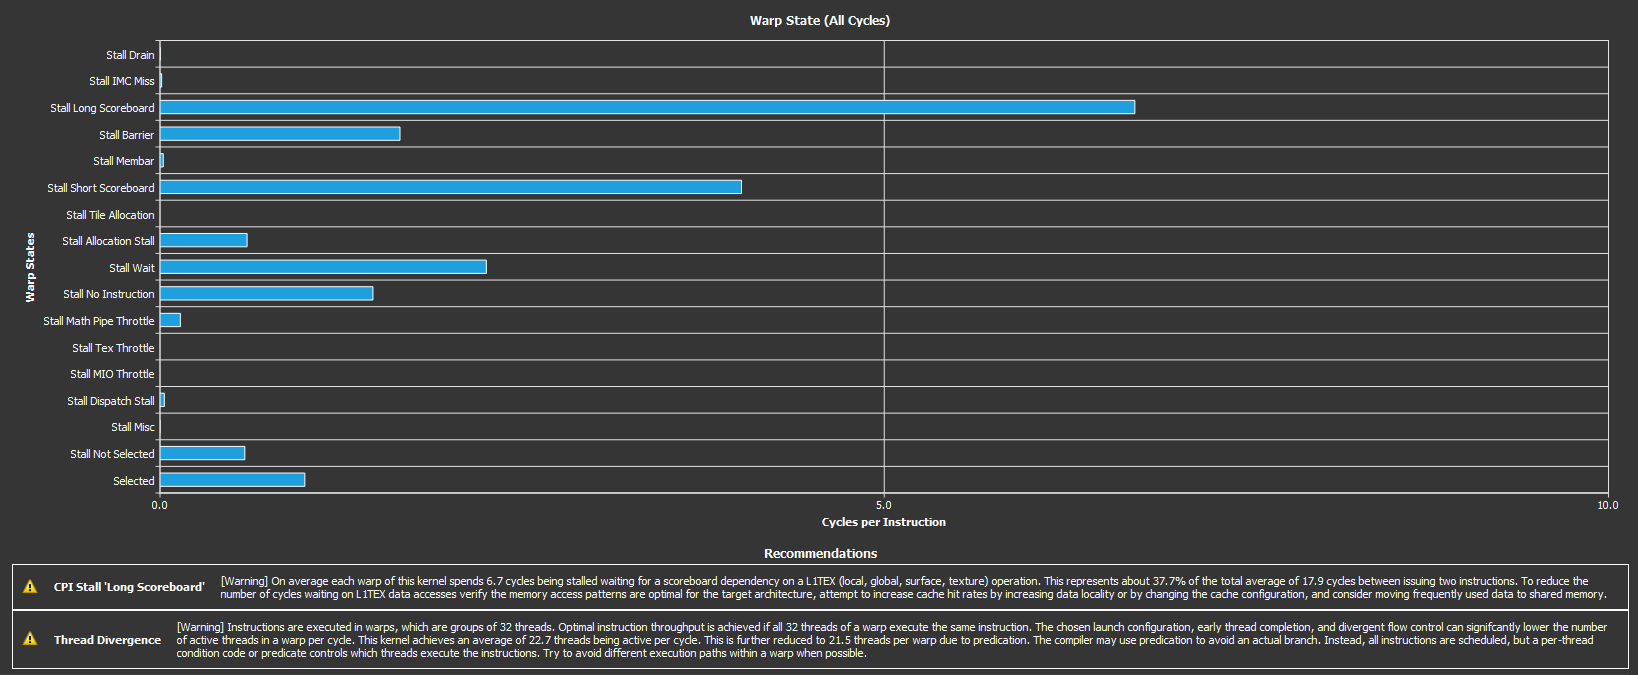
\includegraphics[scale=0.3]{imagenes/som_warp_states.png}
\caption{Análisis de los warps del kernel.}
\label{img:warpssom}
\end{figure}

En la figura \ref{img:warpssom} vemos las dos razones principales que hacen que el \textit{kernel} no funcione más rápido. Una de ellas es la cantidad de accesos a memoria dentro del dispositivo y la otra es la divergencia de las hebras, es decir, situaciones en las que las hebras quieren ejecutar diferentes instrucciones.\\

 Todos los elementos dentro de un bloque que eran utilizados más de una vez fueron cargados en memoria compartida, por lo que, podemos intuir que este problema radica de conflictos que surjan del uso de las operaciones de suma atómica. Encontrar una alternativa mejor que la planteada para el cálculo de los pesos parciales debería de ser la prioridad a la hora de optimizar este algoritmo. \\

 Por otro lado, el segundo problema que destacamos es la divergencia, que se debe principalmente a que, en este ejemplo, trabajamos con 128 hebras por bloque mientras que el número de neuronas es 100, por lo que uno de los \textit{warps} utilizará tan sólo 4 de las 32 hebras. En un caso ideal, el tamaño del mapa tendría un número de neuronas que fuese potencia de 2 (al menos 32). Si tuviésemos garantizado que esto fuese a ocurrir, podríamos eliminar gran parte de los condicionales utilizados, ya que, no sería necesario comprobar si hay más hebras que neuronas, ni habría que rellenar distancias extras con infinito, ni tendríamos que realizar todas las comprobaciones en la reducción para tamaños de bloque superiores al número de neuronas.

\section{Experimentos para evaluar el random forest.}
Para la evaluación de los resultados del \textit{random forest}, hemos utilizado el conjunto de datos SUSY. Para entrenar el \textit{random forest}, se ha usado validación cruzada con 10 iteraciones, es decir, el conjunto de muestras se ha dividido en 10 subconjuntos de muestras del mismo tamaño; en cada iteración, 9 de esos subconjuntos han sido utilizados para entrenar el \textit{random forest} y uno para evaluar los resultados; y, para finalizar, se ha realizado un promedio de los resultados. Para evaluar el modelo, hemos utilizado tres métricas: precisión, que indica el porcentaje de muestras que han sido correctamente clasificadas; el tiempo que tarda en entrenar el algoritmo; y la ganancia de la GPU a la CPU, o sea, cuántas veces es más rápida la tarjeta gráfica que el procesador. \\

Puesto que, tanto la versión para GPU como para CPU utilizan el mismo algoritmo pero, adaptado para las correspondientes arquitecturas, la precisión es un factor relevante a la hora de comprobar si la implementación de los algoritmos es correcta, ya que, en caso de una buena implementación, independientemente de haber usado GPU o CPU, obtendríamos precisiones idénticas, y estos resultados podemos compararlos con los obtenidos en aproximaciones similares en la literatura. \\

Además, durante el proceso de implementación, hemos utilizado otros conjuntos de datos, como Spambase \cite{spambase} o \textit{MAGIC} \cite{magic04}, para comprobar los resultados mientras utilizábamos un único árbol.

Para la evaluación del \textit{random forest} con \textit{SUSY} hemos generado un \textit{random forest} con 12 árboles y hemos utilizado validación cruzada con 10 iteraciones sobre el total de los 5 millones de muestras disponibles en el conjunto de datos. El experimento ha sido realizado múltiples veces, variando la profundidad de 4 a 10. Además, el experimento ha sido repetido 5 veces, anotando los resultados promedios, que podemos observar en la tabla \ref{tab:rf}.\\
\begin{table}[ht]
\centering
\begin{tabular}{@{}l|ll|c|c|@{}}
\cmidrule(l){2-5}
\textit{\textbf{}}                                  & \multicolumn{1}{l|}{\textit{\textbf{GPU}}} & \textit{\textbf{CPU}} & \multicolumn{1}{l|}{\textit{\textbf{GPU vs CPU}}} & \multicolumn{1}{l|}{\textbf{GPU/CPU}} \\ \midrule
\multicolumn{1}{|c|}{\textit{\textbf{Profundidad}}} & \multicolumn{2}{c|}{\textit{\textbf{Tiempo (s)}}}                  & \textit{\textbf{Ganancia}}                        & \textbf{Precisión (\%)}               \\ \midrule
\multicolumn{1}{|l|}{4}                             & 25,58                                      & 27,64                 & 1,08                                              & 75,82                                 \\
\multicolumn{1}{|l|}{5}                             & 26,06                                      & 31,71                 & 1,22                                              & 76,99                                 \\
\multicolumn{1}{|l|}{6}                             & 26,20                                      & 35,30                 & 1,35                                              & 77,44                                 \\
\multicolumn{1}{|l|}{7}                             & 26,45                                      & 38,19                 & 1,44                                              & 78,33                                 \\
\multicolumn{1}{|l|}{8}                             & 27,34                                      & 40,87                 & 1,49                                              & 78,67                                 \\
\multicolumn{1}{|l|}{9}                             & 29,97                                      & 45,85                 & 1,53                                              & 79,02                                 \\
\multicolumn{1}{|l|}{10}                            & 33,63                                      & 48,66                 & 1,45                                              & 79,25                                 \\ \bottomrule
\end{tabular}
\caption{Resultados de Random Forest para SUSY con 12 árboles}
\label{tab:rf}
\end{table}

A diferencia del mapa auto-organizado, podemos observar que, en este caso, los resultados en este modelo se encuentran mucho más ajustados. Para poder realizar una interpretación adecuada de los tiempos de ejecución y la ganancia, hemos de tener en cuenta los siguientes factores:

\begin{itemize}
	\item Dada la implementación realizada, la versión para GPU conseguirá mejores resultados conforme mayor sea el número de elementos a procesar.
	\item El número de árboles utilizados en el \textit{random forest} va a influir en el tiempo de ejecución de la GPU. Conforme mayor sea el número de árboles utilizados, menor será el tamaño de elementos que tenemos garantizados que se procesen a la vez, si estamos usando una única GPU.
	\item Árboles muy profundos afectan de manera negativa a la GPU, debido a que, conforme pasemos al siguiente nivel de profundidad, vamos a tener un mayor número de nodos con un menor número de muestras cada uno o incluso parte de las muestras habrían sido eliminadas en alguna poda, que, limitando la capacidad de aprovechar la máxima capacidad de paralelismo posible.
\end{itemize}

En el ejemplo mostrado en la tabla \ref{tab:rf}, observamos que la versión para GPU nos ofrece una mejora del tiempo de ejecución al usar la GPU. En la profundidad 4, obtenemos el resultado que menos mejora nos ofrece con una diferencia de tan sólo 2 segundos. Mientras que la cantidad de datos sea lo suficientemente grande, una mayor profundidad implica más procesamiento de datos y vamos a obtener una mejor ganancia hasta la profundidad 9, en la que obtenemos la mejor ganancia, siendo la versión para GPU 1,53 veces más rápida que la correspondiente para CPU dándonos una ventaja de 15,88 segundos. En la profundidad 10, observamos cómo esa ganancia empieza a decaer bajando a 1,45 veces más rápido. \\

En el caso de la precisión, una mayor profundidad nos ayuda a obtener mejores resultados, partiendo de un 75,82 \% en la profundidad 4 hasta un 79,25 \% en la profundidad 10. . En comparación con otras aproximaciones de la literatura utilizadas para resolver este problema, la implementación realizada queda considerablemente por detrás del 85-87 \% obtenido utilizado otros modelos \cite{susy}. \\

Para concluir este análisis, podemos determinar que varios factores van a influir en qué situaciones va a ser mejor nuestra aproximación.
\begin{itemize}
\item Para considerar utilizar este modelo hemos de estar trabajando con bases de datos de una combinación de número de muestras y número de atributos considerablemente grandes.
\item El número de árboles utilizados va a influir tanto en la precisión como en el tiempo de ejecución. Por regla generar, un mayor número de árboles va a mejorar la precisión pero va a reducir la velocidad de entrenamiento si se va a utilizar una única GPU. En el caso de disponer de un clúster, tener un número de GPUs igual al número de árboles nos permitiría obtener los mejores resultados, siempre y cuando el tiempo de comunicación entre los nodos del clúster no sea demasiado alto.
\item Dependiendo del problema a resolver podremos variar el número de árboles o la profundidad que queremos usar para entrenar. Además, mientras que en el ejemplo propuesto obtenemos una precisión por debajo de otras alternativas, en ejemplos más simples, como en \textit{Spambase} \cite{spambase} o \textit{MAGIC} \cite{magic04} obtenemos precisiones muy competentes con otros resultados encontrados en la literatura (un 91,9 \% y un 82,4 \%, respectivamente, para profundidad 10).
\end{itemize}

\subsection{Resultados del uso del profiler sobre la versión final del algoritmo.}
En el caso del árbol de decisión desarrollado, el principal cuello de botella es la necesidad de lanzar una gran cantidad de \textit{kernels} muy rápidos que no hemos sido capaces de compactar para evitar el \textit{overhead} de cada lanzamiento de un kernel. Para evitarlo, hemos utilizado algunas técnicas para evitar este problema como el uso de \textit{streams} concurrentes o la combinación de múltiples \textit{kernels} (scan con cálculo del criterio de Gini y scan con el cálculo de las nuevas posiciones en la lista de atributos). Cabe también destacar, que otra alternativa a evaluar para solucionar este problema es el uso del paralelismo dinámico de \textit{CUDA}, que permite lanzar un kernel desde otro, sin embargo, no tenemos acceso a esa característica usando \textit{Python}.\\

Puesto que hay una alta variedad de \textit{kernels}, que son invocados frecuentemente, vamos a observar la siguiente gráfica, en la que vemos el porcentaje del tiempo de ejecución que se dedica a cada tarea en una reproducción del experimento, con una base de datos de 100000 muestras aleatorias con 18 atributos y generando un árbol de profundidad 10.

\begin{figure}[ht]
\centering
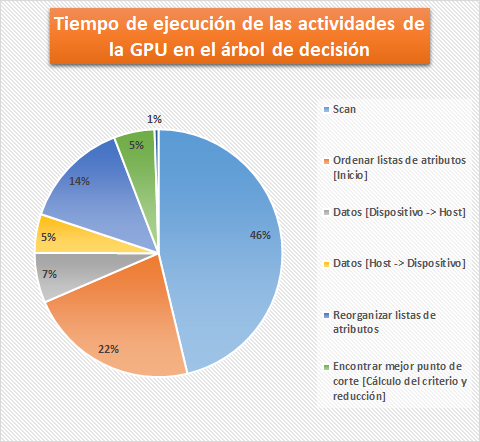
\includegraphics[scale=0.8]{imagenes/profiletreequesito.png}
\caption{Análisis de los kernels ejecutados.}
\label{img:quesito}
\end{figure}

En primer lugar, la operación que más porcentaje de tiempo lleva es la operación más costosa, la organización de la listas de atributos inicial que toma un 27 \% del tiempo total de ejecución de la GPU, correspondiente al algoritmo de ordenación de CuPy. Esta operación, que junto a la inicialización de la lista de atributos supone el inicio del algoritmo, acumulado un 29 \% del tiempo usado. Una posible vía de mejora es evaluar si una implementación propia del algoritmo de ordenación nos proporcionaría resultados mejores. En caso de realizar una implementación propia, podríamos combinar con facilidad la inicialización de las listas de atributos con el algoritmo de ordenación. \\

En segundo lugar, tenemos un empate al 20 \% entre la reducción utilizada para calcular el criterio de Gini y la reorganización de la listas de atributos. La operación de reducción es invocada para todos los nodos activos mientras que la reorganización de atributos es realizada una vez por nivel de profundidad. \\

La implementación de la reducción para este algoritmo sigue una estructura similar a la operación de \textit{scan}. Ésta, hace uso de operaciones intrínsecas de \textit{warps} y de operaciones atómicas para calcular el mínimo global entre los bloques. Otra alternativa probada fue el lanzamiento de otro kernel para el cálculo de los resultados globales, pero resultó ligeramente más lenta que el uso de las operaciones atómicas. Otra opción a evaluar, sería el uso del paralelismo dinámico, pero como comentamos previamente, no podemos acceder a esa característica desde \textit{Numba}.\\

La reorganización de la listas de atributos es una operación de transferencia de memoria dentro del dispositivo. En primer lugar, los datos son movidos a \textit{arrays} temporales y, una vez finalizado el proceso, se sobrescriben los datos en las nuevas posiciones. Dentro del dispositivo \textit{CUDA}, estas transferencias de memoria son considerablemente rápidas, especialmente cuando los datos siguen algún patrón de adyacencia, como sucede al rellenar los arrays temporales. Sin embargo, en el caso de los accesos a memoria aleatorios, como ocurre en la fase de escritura, el tiempo de acceso va a ser mucho más lento, que queda manifestado en que, de ese 20 \%, un 5,1 \% se corresponde a la primera fase y el resto a la segunda. \\

Por último, vamos a analizar las tres operaciones relacionadas con la primitiva de \textit{scan}, que son las siguientes en la gráfica. La operación de \textit{scan} es usada dos veces por nodo activo, una primera vez para calcular el criterio de Gini y, una segunda vez, para calcular qué transferencias de memoria permiten mantener el orden de los atributos sin tener que volver a usar el algoritmo de ordenación, haciendo de ella la operación que es invocada el mayor número de veces por ejecución del algoritmo. A diferencia del caso de la reducción, en vez de utilizar operaciones atómicas, usamos el lanzamiento de un nuevo \textit{kernel} para realizar el cálculo global del \textit{scan}. Este cambio se debe a que, dadas las necesidades de lanzar otros \textit{kernels} para ejecutar el algoritmo sin paralelismo dinámico hemos podido combinar el cálculo del \textit{scan} global con la operación posterior. La parte que realiza el cálculo de la primitiva \textit{scan} para cada bloque representa un 15 \% del tiempo de ejecución de la GPU mientras que el \textit{kernel} que termina la primitiva y calcula el criterio de Gini conlleva un 8 \% del tiempo y el cálculo de los nuevas posiciones para ordenar un 5 \%. Puesto que, ambos \textit{kernels} parten de la misma operación (realizar el \textit{scan} global) podemos deducir que la complejidad aritmética del cálculo del criterio de Gini es superior a la del cálculo de las nuevas posiciones.\\

Aunque el análisis previo nos facilita saber qué \textit{kernel} nos interesaría optimizar primero es importante observar un resultado más genérico obtenido en el \textit{profile} nos indica que durante los 0,25 segundos que ha tardado en entrenarse el árbol sólo 0,1 segundos han sido usados para realizar los cálculos, proporcionado un porcentaje de utilización de la GPU del 40 \%. Este problema deriva principalmente del \textit{overhead} de tener que lanzar múltiples \textit{kernels}, que viene dada por la necesidad de evaluar múltiples nodos independientes, que, además, han de ser sincronizados al terminar cada nivel de profundidad para reorganizar las listas de atributos y poder pasar al siguiente nivel.
\chapter{Conclusiones y trabajos futuros.}
%\chapter{Estado del arte.}
%\chapter{Mapas autoorganizados.}
\section{Definición.}
Los mapas autoorganizados \textit{Self Organizing Map}, también llamados mapa autoorganizados de características \textit{Self Organizing Feature Map} o redes neuronales de Kohonen son un modelo neuronal de aprendizaje competitivo y no supervisado propuesto por \textit{Teuvo Kohonen} a principios de la década de 1980.\\

Al ser un modelo de aprendizaje no supervisado, se encarga de descrubir patrones iguales en las muestras y agruparlos basandose en la información de las características. 

\section{Arquitectura de una mapa autoorganizado.}
La arquitectura de este tipo de redes neuronales está formada por dos capas totalmente interconectadas. Una capa de entrada y una capa de salida (también llamada capa de Kohonen, capa competitiva o capa de aprendizaje). \\

La capa de entrada tiene el mismo número de nodos que el número de características que tiene cada muestra de entrada.\\

La capa de salida está compuesta por una estructura con $X$ neuronas, habitaulmente colocadas en una matriz bidimensional, aunque no tiene por qué ser así, donde cada una de estas neuronas tiene asociada un vector de pesos $W$ que une cada uno de los nodos de entrada con una neurona de la capa de salida.
\begin{figure}
\centering
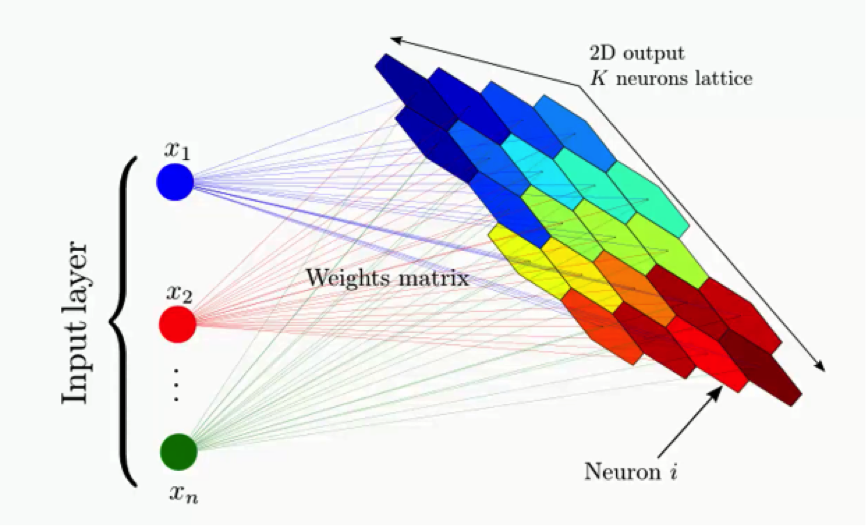
\includegraphics[width=0.8\textwidth]{imagenes/arquitectura_som.png}
\caption{Esquema de una red neuronal de Kohonen.}
\end{figure}
\section{Proceso de entrenamiento de un mapa autoorganizado.}
\textit{En la explicación de este algoritmo se asume que la capa de salida es una matriz bidimensional, como se ha comentado antes, esto no tiene que ocurrir aunque es lo más común.}\\

En primer lugar, se \textbf{inicializan} \textbf{los pesos} asociados a la capa de salida. Lo más habitual, es tomar dichos pesos de una distribución aleatoria.
Para un correcto funcionamiento dichos pesos deben estar normalizados entre 0 y 1. En nuestro caso, hemos tomado los pesos de una distribución aleatoria uniforme en el intervalo $[0, 1)$.\\

El proceso de entrenamiento que se presenta a continuación \textbf{se repite hasta que se alcanza el número de iteraciones máximo}, determinado por el parámetro $\lambda$. La variable $t$ representa cada una de las iteraciones.\\

Después, para cada una de las muestras, $X$, sacadas de la distribución de muestras, de forma aleatoria, se realizan los siguientes pasos: \\\\
1 - Se \textbf{calcula la distancia euclídea} entre la muestra $X$ y cada una de las neuronas de la capa de salida.\\
$$distancia(X) = || W - X ||$$\\
2 - Se \textbf{busca la neurona que ha obtenido una menor distancia}. Esta neurona es considerada la neurona ganadora o BMU \textit{(Best Matching Unit)}.\\
$$BMU_X = argmin_{W_{i, j}} \; distancia(X) = argmin_{W_{i, j}} || W - X ||$$\\
3 - Se realiza un \textbf{proceso de actualización de las matrices de pesos} en base a lo obtenido anteriormente, según la siguiente fórmula.\\
$$ W_{i, j}^{(t+1)} = W_{i, j}^{(t)} + \Delta {W_{i,j}} $$\\

La actualización depende tanto de la distancia de la muestra al vector de pesos como de otros dos parámetros: la tase de aprendizaje y una función de vecindario.\\

$$\Delta W_{i,j} = \eta(t)\delta_f(i,j)(X-W_{i,j})$$\\

La función $\delta_f(i,j)$ es la función de vecindario y, en nuestra se calcula conforme a la siguiente ecuación:\\

$$\delta_f(i,j) = e ^{-\frac{||BMU_X-(i,j)||^2}{2\sigma(t)^2}}. $$\\

Al tratar con una potencia con exponente negativo, un mayor valor absoluto de dicho exponente nos proporciona una valor de $\delta_f(i,j)$ menor. Por eso en el numerador se tiene en cuenta la distancia que hay entre la mejor neurona y la neurona actual. En el denominador se utiliza un parámetro de control $\sigma$que nos permite controlar la distancia que estamos considerando.\\\\

Normalmente, este parámetro, durante un primer número de iteraciones previamente proporcionado, de las consideradas en el proceso de entrenamiento, es inicializado a un valor alto $\sigma_0$ que decrece de manera exponencial conforme a otro parámetro de control $\tau$.


Una vez ha finalizado esa primera fase (han pasado $z$ iteraciones) se van refinando los resultados con un valor fijo mucho más bajo $\sigma_f$.\\


$$\sigma(t) = \left\{
\begin{array}{ll}
\sigma_0e^{-\frac{t}{\tau}} & si \;\;t < z\\
\sigma_f & si  \;\; t\geq z
\end{array}
\right.
$$\\

Para la tasa de aprendizaje se sigue una aproximación similar, la tasa de aprendizaje durante la primera fase está inicializada a un valor $\eta_0$ decreciendo conforme a una gaussiana y, una vez pasado un número de iteraciones, es fijado a un valor $\eta_f$. \\
$$\sigma(t) = \left\{
\begin{array}{ll}
\eta_0e^{-\frac{t}{\tau}} & si \;\;t < z\\
\eta_f & si  \;\; t\geq z
\end{array}
\right.$$\\

Así pues, este algoritmo acerca los pesos del vecindario de la BMU hacia la nueva muestra introducida para parecerse más a la misma. Esto lo hace teniendo en cuenta un vecindario alrededor de la BMU que decrece exponencialmente conforme pasa un número de iteraciones hasta quedarse fijo y una tasa de aprendizaje que también decrece exponencialmente hasta permanecer constante. \\Esto permite una primera fase de entrenamiento, con cambios más bruscos en la que se adaptan los valores completamente aleatorios para encontrar agrupamientos razonables. Conforme avanza dicha fase esos valores van decreciendo, hasta que quedan fijados permitiendo a la red neuronal refinar los agrupamientos obtenidos hasta ese momento.



\section{Implementación en CUDA.}
Antes de realizar la primera implementación en CUDA, analizamos las posibilidades de paralelización que nos aporta el algoritmo así como los accesos a memoria requeridos para utilizar las herramientas que cuda nos proporciona de la forma más eficiente posible.

\subsection{Grado de paralelismo.}
El algoritmo muestra una posibilidad de implementarlo de forma paralela innata. Cada vez que una muestra es tomada de la entrada todas las neuronas realizan las mismas operaciones con esa entrada. Por ello, la componente principal que va a determinar el grado de paralelismo que podríamos alcanzar como máximo viene dado por el número de neuronas que hay en la capa de salida. \\

Otra opción que sería interesante sería que el paralelismo dependiera del número de muestras procesadas, ya que, es mucho más frecuente a la hora de utilizar este tipo de modelos, especialmente al aplicarlos con el fin de realizar \textit{clustering} (agrupamiento de datos) o reducción de dimensionalidad que el número de muestras sea considerablemente superior al número de neuronas (grupos) que se desean obtener en la capa de salida. \\

Sin embargo, la dependencia de datos existente para actualizar la matriz de pesos en cada iteración genera una barrera de comunicación que evita que podamos plantear una solución eficiente del algoritmo estudiando basándonos en las muestras.

\subsection{Uso de memoria.}
En esta sección vamos a analizar las operaciones relacionadas con la memoria para poder tomar decisiones óptimas con respecto a ellas. \\

\underline{Transferencia de elementos del host al dispositivo.}\\
Cada vez que se invoca uno de los kernels utilizados para la resolución del algoritmo acabamos de obtener una nueva muestra dentro de una iteración. Para poder aprovechar la gran capacidad de paralelismo de la GPU es necesario que dichos elementos se encuentren la GPU, por ello, en esta implementación vamos a mover todo el conjunto de muestras al dispositivo antes de empezar a calcular el algoritmo, evitando así que se interrumpa la ejecución constante del dispositivo para recibir nuevas entradas a través del PCI Express 3.0.

Los parámetros de control, se mantendrán todos en la CPU y será necesario enviarlos para el kernel que se encargue de actualizar la matriz de pesos.\\

\underline{Uso de memoria compartida.}\\
El uso de la memoria compartida en una GPU es fundamental para poder obtener los mejores resultados. Esta memoria compartida es mucho más rápida que la memoria global del sistema ya que, en vez de hacer uso de la DRAM del dispositivo, los elementos de esta memoria se alojan en la caché L1 de la tarjeta permitiendo un acceso tanto para escritura como para lectura muy superior pero limitando a 48 KB el máximo de elementos que se pueden alojar por bloque de hebras en la misma.

En el algoritmo propuesto encontramos dos operaciones en las que podemos hacer uso de la memoria compartida.

\begin{itemize}
	\item A la hora de calcular la distancia euclídea, podemos guardar la muestra que estamos evaluando en memoria compartida, asegurándonos de que esta permanezca en la caché.
	\item A la hora de buscar el índice de la menor distancia, que se va a realizar mediante una técnica de reducción y que, por tanto, conlleva el uso de la memoria compartida para obtener buenos resultados.
\end{itemize}

\underline{Uso de la memoria del dispositivo.}\\
Todos los elementos generados en el dispositivo, se mantendrán en el mismo sin necesidad de ser transladados al host, salvo la matriz de pesos solución que una vez finalizada la ejecución del algoritmo se enviará al host. \\

\subsection{Kernels a desarrollar.}
Para obtener los mejores resultados hemos de intentar lanzar el menor número posible de kernels para evitar así los pequeños overheads que se dan para lanzar los mismos. Sin embargo, la naturaleza del algoritmo, que repite el proceso constantemente dificulta esta labor. \\

Antes de iniciar el bucle del algoritmo lanzaremos el primer kernel.\\

\underline{I - Inicialización aleatoria de pesos \textit{(cuda\_init\_weights)}.}\\

En el primer kernel vamos a inicializar aleatoriamente el array de pesos con valores sacados de una distribución uniforme de números reales en coma flotante entre 0 y 1. La generación de números aleatorios se realiza utilizando funciones que nos proporciona la librería Numba, cuya implementación se basa en el método de Box-Muller. \\\\

Este array de una única dimensión representa una estructura tridimensional basado en las filas de la matriz, las columnas de la matriz y la dimensión de los vectores de pesos.\\\\\\

En cada iteración del algoritmo se ejecuta lo siguiente:\\

\underline{II - Selección aleatoria de las muestras a usar \textit{(en CPU)}}\\
Puesto que el tamaño de muestras que se toma por iteración no tiende a ser muy grande, hemos optado por realizar esta opción en la CPU.\\

\underline{III - Cálculo de la distancia euclídea. \textit{(cuda\_euclidean\_distance)}} \\
Este kernel recibe una muestra y calcula la distancia euclídea de esa muestra con todos los elementos de la matriz de pesos. Para hacerlo de una manera más eficiente primero se introduce la muestra en memoria compartida y luego se calcula la distancia.

El array en el que se guardan las distancias resultantes permanece siempre en la memoria del dispositivo y es reutilizado de una iteración a otra. \\

\underline{IV - Encontrar menor distancia \textit{(amin() cuBLAS.)}} \\
En principio para solucionar este problema habíamos planteado una reducción. La reducción es una técnica común utilizada para computar eficientemente en una GPU una operación binaria que cumple la propiedad asociativa sobre todos los elementos de un array. El ejemplo más habitual de ello, es la suma. Puesto que la operación binaria mínimo cumple ese prerrequisito hemos planteado y desarrollado la solución con una reducción en la que tenemos en cuenta la dupla que conforman el valor y su índice en el array.

Este ha sido el objeto de más dificultad de esta implementación y, aunque hemos conseguido una implementación considerablemente eficiente especialmente ante una implementación secuencial, hemos considerarlo sustituirlo por el método amin() de la librería altamente optimizada de cuBLAS que calculaba los resultados entre 2 y 4 veces más rápido (dependiendo del tamaño de la entrada), que nuestra implementación.\\

\underline{ V - Actualización de la matriz de pesos \textit{(cuda\_bmu\_update)}} \\
Este kernel recibe los parámetros de control y aplica la actualización de los pesos conforme a lo descrito en la fase de actualización del algoritmo explicado en la sección anterior (3.3).

%\chapter{Árboles de decisión.}

Un árbol de decisión es un modelo de aprendizaje automático no lineal que permite resolver los problemas de manera jerárquica. Una vez el árbol es construido el árbol consta de dos tipos de nodos: los nodos de decisión y los nodos terminales. Los \textbf{nodos de decisión}, son reglas que nos idican cómo hemos de navegar el árbol para clasificar una muestra. Lo habitual es que dicho nodo esté asociado a una carácterística del problema y un valor de tal manera que si la condición se cumple, tomamos un camino y, en caso contrario, tomamos el otro. Una vez alcanzamos un \textbf{nodo terminal} (correspondientes a las hojas de los árboles), conocemos la categoría a la que corresponde una muestra.\\\\

La mayoría de los algoritmos secuenciales utilizan metodologías de tipo voraz \textit{(greedy)} para la generación de manera recursiva de la estructura del árbol. Dentro de esta categoría encontramos los algoritmos más conocidos como ID3, C4.5 y CART.

%\input{capitulos/01_Introduccion}
%
%\input{capitulos/02_EspecificacionRequisitos}
%
%\input{capitulos/03_Planificacion}
%
%\input{capitulos/04_Analisis}
%
%\input{capitulos/05_Diseno}
%
%\input{capitulos/06_Implementacion}
%
%\input{capitulos/07_Pruebas}
%
%\input{capitulos/08_Conclusiones}
%
%%\chapter{Conclusiones y Trabajos Futuros}
%
%
%%\nocite{*}
%\bibliographystyle{miunsrturl} 
\bibliographystyle{IEEEtran} 
\bibliography{bibliografia/bibliografia}\addcontentsline{toc}{chapter}{Bibliografía}
%

%\input{apendices/manual_usuario/manual_usuario}
%\chapter{ESPECIFICACIONES DEL SISTEMA}
Aquí se especifican las características del sistema utilizado para las pruebas.

\begin{itemize}
\item \textbf{Placa Base:} MSI B450M Bazooka
\item \textbf{Sistema Operativo:} Windows 10 64 bits
\item \textbf{CPU:} AMD Ryzen 5 2600X
\item \textbf{RAM:} Kingston HyperX Fury Black DDR4 2400 MHz PC4-19200 8GB CL15
\item \textbf{GPU}: \underline{Zotac GeForce GTX 1060 AMP! Edition}
\subitem \textbf{Núcleos CUDA}: 1280
\subitem \textbf{Frecuencia del procesador:} 1556 MHz (1771 MHz Boost)
\subitem \textbf{Frecuencia de la memoria:} 8 GHz
\subitem \textbf{Memoria}: 6 GB DDR5
\subitem \textbf{Bus de memoria:} 192-bit
\subitem \textbf{Compute Capability:} 6.1


\end{itemize}
%\input{glosario/entradas_glosario}
% \addcontentsline{toc}{chapter}{Glosario}
% \printglossary

\thispagestyle{empty}

\end{document}


 